\documentclass[twoside]{book}

% Packages required by doxygen
\usepackage{fixltx2e}
\usepackage{calc}
\usepackage{doxygen}
\usepackage[export]{adjustbox} % also loads graphicx
\usepackage{graphicx}
\usepackage[utf8]{inputenc}
\usepackage{makeidx}
\usepackage{multicol}
\usepackage{multirow}
\PassOptionsToPackage{warn}{textcomp}
\usepackage{textcomp}
\usepackage[nointegrals]{wasysym}
\usepackage[table]{xcolor}

% Font selection
\usepackage[T1]{fontenc}
\usepackage[scaled=.90]{helvet}
\usepackage{courier}
\usepackage{amssymb}
\usepackage{sectsty}
\renewcommand{\familydefault}{\sfdefault}
\allsectionsfont{%
  \fontseries{bc}\selectfont%
  \color{darkgray}%
}
\renewcommand{\DoxyLabelFont}{%
  \fontseries{bc}\selectfont%
  \color{darkgray}%
}
\newcommand{\+}{\discretionary{\mbox{\scriptsize$\hookleftarrow$}}{}{}}

% Page & text layout
\usepackage{geometry}
\geometry{%
  a4paper,%
  top=2.5cm,%
  bottom=2.5cm,%
  left=2.5cm,%
  right=2.5cm%
}
\tolerance=750
\hfuzz=15pt
\hbadness=750
\setlength{\emergencystretch}{15pt}
\setlength{\parindent}{0cm}
\setlength{\parskip}{3ex plus 2ex minus 2ex}
\makeatletter
\renewcommand{\paragraph}{%
  \@startsection{paragraph}{4}{0ex}{-1.0ex}{1.0ex}{%
    \normalfont\normalsize\bfseries\SS@parafont%
  }%
}
\renewcommand{\subparagraph}{%
  \@startsection{subparagraph}{5}{0ex}{-1.0ex}{1.0ex}{%
    \normalfont\normalsize\bfseries\SS@subparafont%
  }%
}
\makeatother

% Headers & footers
\usepackage{fancyhdr}
\pagestyle{fancyplain}
\fancyhead[LE]{\fancyplain{}{\bfseries\thepage}}
\fancyhead[CE]{\fancyplain{}{}}
\fancyhead[RE]{\fancyplain{}{\bfseries\leftmark}}
\fancyhead[LO]{\fancyplain{}{\bfseries\rightmark}}
\fancyhead[CO]{\fancyplain{}{}}
\fancyhead[RO]{\fancyplain{}{\bfseries\thepage}}
\fancyfoot[LE]{\fancyplain{}{}}
\fancyfoot[CE]{\fancyplain{}{}}
\fancyfoot[RE]{\fancyplain{}{\bfseries\scriptsize Generated by Doxygen }}
\fancyfoot[LO]{\fancyplain{}{\bfseries\scriptsize Generated by Doxygen }}
\fancyfoot[CO]{\fancyplain{}{}}
\fancyfoot[RO]{\fancyplain{}{}}
\renewcommand{\footrulewidth}{0.4pt}
\renewcommand{\chaptermark}[1]{%
  \markboth{#1}{}%
}
\renewcommand{\sectionmark}[1]{%
  \markright{\thesection\ #1}%
}

% Indices & bibliography
\usepackage{natbib}
\usepackage[titles]{tocloft}
\setcounter{tocdepth}{3}
\setcounter{secnumdepth}{5}
\makeindex

% Hyperlinks (required, but should be loaded last)
\usepackage{ifpdf}
\ifpdf
  \usepackage[pdftex,pagebackref=true]{hyperref}
\else
  \usepackage[ps2pdf,pagebackref=true]{hyperref}
\fi
\hypersetup{%
  colorlinks=true,%
  linkcolor=blue,%
  citecolor=blue,%
  unicode%
}

% Custom commands
\newcommand{\clearemptydoublepage}{%
  \newpage{\pagestyle{empty}\cleardoublepage}%
}

\usepackage{caption}
\captionsetup{labelsep=space,justification=centering,font={bf},singlelinecheck=off,skip=4pt,position=top}

%===== C O N T E N T S =====

\begin{document}

% Titlepage & ToC
\hypersetup{pageanchor=false,
             bookmarksnumbered=true,
             pdfencoding=unicode
            }
\pagenumbering{alph}
\begin{titlepage}
\vspace*{7cm}
\begin{center}%
{\Large Transit Network Model }\\
\vspace*{1cm}
{\large Generated by Doxygen 1.8.14}\\
\end{center}
\end{titlepage}
\clearemptydoublepage
\pagenumbering{roman}
\tableofcontents
\clearemptydoublepage
\pagenumbering{arabic}
\hypersetup{pageanchor=true}

%--- Begin generated contents ---
\chapter{Main Page}
\label{index}\hypertarget{index}{}A realtime model of a public transport network.

An program which runs indefinitely, modeling the realtime state of all vehicles in the transit network. These are in turn used to model the realtime state of the network itself (road speeds), and finally arrival time predictions made for each vehicle/stop combination.


\begin{DoxyItemize}
\item \hyperlink{transit__network__model_8cpp}{transit\+\_\+network\+\_\+model.\+cpp} 
\end{DoxyItemize}
\chapter{Transit Network Model}
\label{md_README}
\Hypertarget{md_README}
Three parts, running in real time\+:
\begin{DoxyEnumerate}
\item particle filter for vehicle location and speed
\item Kalman filter for transit road network state (speed)
\item travel-\/ and arrival-\/time predictions for each vehicle/stop combination in the network
\end{DoxyEnumerate}

\subsubsection*{1. Particle Filter}

{\bfseries IN}\+: G\+T\+FS realtime protobuf feed

{\bfseries O\+UT}\+: (updated) vehicle objects with updated particle states

\subsubsection*{2. Kalman filter}

{\bfseries IN}\+: particle filter state estimates, road state at time {\ttfamily now -\/ delta}

{\bfseries O\+UT}\+: road state at time {\ttfamily now}

\subsubsection*{3. Predictions}

{\bfseries IN}\+: particle filter state estimates, road state estimates

{\bfseries O\+UT}\+: E\+TA to remaining stops along route



 \subsection*{Dependencies}


\begin{DoxyItemize}
\item C\+Make
\item (optional) Doxygen (for making the Documentation)
\item (optional) https\+://github.com/google/protobuf/blob/master/src/\+R\+E\+A\+D\+M\+E.\+md \char`\"{}\+Google protobuf compiler `protoc`\char`\"{}
\end{DoxyItemize}

\subsection*{To-\/do}


\begin{DoxyItemize}
\item Application to run indefinitely
\item Use a {\ttfamily Vehicle} object concept with
\begin{DoxyItemize}
\item {\ttfamily vector$<$Particle$>$ (N)}
\item {\ttfamily void update (gtfs\+::\+Vehicle\+Position, gtfs\+::\+Trip\+Update)}\+: adjust the position, arrival/departure times etc, trigger particle transitions
\item {\ttfamily void resample (N)}\+: perform particle filter weighted resample
\item properties {\ttfamily vehicle\+\_\+id}, {\ttfamily timestamp}, {\ttfamily trip\+\_\+id}, {\ttfamily route\+\_\+id}, {\ttfamily position}, {\ttfamily stop\+\_\+sequence}, {\ttfamily arrival\+\_\+time}, {\ttfamily departure\+\_\+time}
\end{DoxyItemize}
\item And the particles work in memory only
\begin{DoxyItemize}
\item {\ttfamily Particle}
\begin{DoxyItemize}
\item {\ttfamily void initialize ()}
\item {\ttfamily void transition ()}
\item {\ttfamily void calc\+\_\+likelihood ()}\+: uses parent Vehicle
\item {\ttfamily void calc\+\_\+weight ()}
\item properties {\ttfamily distance}, {\ttfamily velocity}, {\ttfamily stop\+\_\+index}, {\ttfamily arrival\+\_\+time}, {\ttfamily departure\+\_\+time}, {\ttfamily segment\+\_\+index}, {\ttfamily queue\+\_\+time}, {\ttfamily begin\+\_\+time}, {\ttfamily likelihood}, {\ttfamily weight}
\end{DoxyItemize}
\end{DoxyItemize}
\item Similar concept for network route segments
\begin{DoxyItemize}
\item {\ttfamily Segment}
\begin{DoxyItemize}
\item {\ttfamily vector$<$Path$>$ shape}\+: the G\+PS coordinates and cumulative distance of segment shape
\item {\ttfamily double speed}
\item {\ttfamily void update ()}\+: perform Kalman filter update, using particle summaries (?)
\end{DoxyItemize}
\end{DoxyItemize}
\item The G\+T\+FS information can either be
\begin{DoxyItemize}
\item loaded into an S\+Q\+Lite database, or
\item loaded into a M\+E\+M\+O\+RY table via My\+S\+QL
\end{DoxyItemize}
\item Vehicle state summaries can be written to a file (?)
\item Making information available (via server) -\/ road segment speeds + arrival time predictions
\begin{DoxyItemize}
\item database (with no foreign key checks, and no transaction?)
\end{DoxyItemize}
\end{DoxyItemize}

(?) best way of collecting vehicle/segment data
\begin{DoxyItemize}
\item sequentially append speed estimates to {\ttfamily Segment}, then periodically update and clear?
\item write to file? (makes keeping history easier?)
\end{DoxyItemize}

\subsection*{Project Structure}


\begin{DoxyItemize}
\item {\ttfamily bin}
\begin{DoxyItemize}
\item {\ttfamily transit\+\_\+network\+\_\+model}\+: the application that\textquotesingle{}ll run \textquotesingle{}infinitely\textquotesingle{}
\item {\ttfamily load\+\_\+gtfs}\+: this will load G\+T\+FS when updates released, and do the segmentation
\end{DoxyItemize}
\item {\ttfamily src}
\begin{DoxyItemize}
\item {\ttfamily \hyperlink{transit__network__model_8cpp}{transit\+\_\+network\+\_\+model.\+cpp}}\+: mostly just a wrapper for {\ttfamily while (T\+R\+UE) \{ ... \}}
\item {\ttfamily laod\+\_\+gtfs.\+cpp}
\end{DoxyItemize}
\item {\ttfamily include}
\begin{DoxyItemize}
\item {\ttfamily gtfs}\+: descriptions of the gtfs objects (??)
\begin{DoxyItemize}
\item {\ttfamily \hyperlink{classgtfs_1_1Vehicle}{gtfs\+::\+Vehicle}} a vehicle object
\item {\ttfamily \hyperlink{classgtfs_1_1Particle}{gtfs\+::\+Particle}}
\end{DoxyItemize}
\item {\ttfamily gps}\+: methods for G\+PS coordinates (distance, etc)
\item {\ttfamily particle\+\_\+filter}\+: the particle filter model
\item {\ttfamily kalman\+\_\+filter}\+: the Kalman filter model
\item {\ttfamily segmentation}\+: the segmentation algorithm for (new) segments
\item {\ttfamily database}\+: any database methods (connection, S\+E\+L\+E\+CT, I\+N\+S\+E\+RT, etc)
\end{DoxyItemize}
\item {\ttfamily lib}
\begin{DoxyItemize}
\item {\ttfamily gtfsrealtime.\+proto}\+: the schema for G\+T\+FS protobuf feed 
\end{DoxyItemize}
\end{DoxyItemize}
\chapter{Namespace Index}
\section{Namespace List}
Here is a list of all documented namespaces with brief descriptions\+:\begin{DoxyCompactList}
\item\contentsline{section}{\hyperlink{namespacegps}{gps} }{\pageref{namespacegps}}{}
\item\contentsline{section}{\hyperlink{namespacegtfs}{gtfs} }{\pageref{namespacegtfs}}{}
\item\contentsline{section}{\hyperlink{namespacenlohmann}{nlohmann} \\*Namespace for Niels Lohmann }{\pageref{namespacenlohmann}}{}
\item\contentsline{section}{\hyperlink{namespacenlohmann_1_1detail}{nlohmann\+::detail} \\*Unnamed namespace with internal helper functions }{\pageref{namespacenlohmann_1_1detail}}{}
\item\contentsline{section}{\hyperlink{namespacesampling}{sampling} }{\pageref{namespacesampling}}{}
\end{DoxyCompactList}

\chapter{Class Index}
\section{Class List}
Here are the classes, structs, unions and interfaces with brief descriptions\+:\begin{DoxyCompactList}
\item\contentsline{section}{\hyperlink{structnlohmann_1_1adl__serializer}{nlohmann\+::adl\+\_\+serializer$<$ typename, typename $>$} \\*Default J\+S\+O\+N\+Serializer template argument }{\pageref{structnlohmann_1_1adl__serializer}}{}
\item\contentsline{section}{\hyperlink{classnlohmann_1_1basic__json}{nlohmann\+::basic\+\_\+json$<$ Object\+Type, Array\+Type, String\+Type, Boolean\+Type, Number\+Integer\+Type, Number\+Unsigned\+Type, Number\+Float\+Type, Allocator\+Type, J\+S\+O\+N\+Serializer $>$} \\*Class to store J\+S\+ON values }{\pageref{classnlohmann_1_1basic__json}}{}
\item\contentsline{section}{\hyperlink{structnlohmann_1_1detail_1_1conjunction}{nlohmann\+::detail\+::conjunction$<$... $>$} }{\pageref{structnlohmann_1_1detail_1_1conjunction}}{}
\item\contentsline{section}{\hyperlink{structnlohmann_1_1detail_1_1conjunction_3_01B1_01_4}{nlohmann\+::detail\+::conjunction$<$ B1 $>$} }{\pageref{structnlohmann_1_1detail_1_1conjunction_3_01B1_01_4}}{}
\item\contentsline{section}{\hyperlink{structnlohmann_1_1detail_1_1conjunction_3_01B1_00_01Bn_8_8_8_01_4}{nlohmann\+::detail\+::conjunction$<$ B1, Bn... $>$} }{\pageref{structnlohmann_1_1detail_1_1conjunction_3_01B1_00_01Bn_8_8_8_01_4}}{}
\item\contentsline{section}{\hyperlink{classgps_1_1Coord}{gps\+::\+Coord} }{\pageref{classgps_1_1Coord}}{}
\item\contentsline{section}{\hyperlink{classsampling_1_1exponential}{sampling\+::exponential} }{\pageref{classsampling_1_1exponential}}{}
\item\contentsline{section}{\hyperlink{structnlohmann_1_1detail_1_1external__constructor}{nlohmann\+::detail\+::external\+\_\+constructor$<$ value\+\_\+t $>$} }{\pageref{structnlohmann_1_1detail_1_1external__constructor}}{}
\item\contentsline{section}{\hyperlink{structnlohmann_1_1detail_1_1external__constructor_3_01value__t_1_1array_01_4}{nlohmann\+::detail\+::external\+\_\+constructor$<$ value\+\_\+t\+::array $>$} }{\pageref{structnlohmann_1_1detail_1_1external__constructor_3_01value__t_1_1array_01_4}}{}
\item\contentsline{section}{\hyperlink{structnlohmann_1_1detail_1_1external__constructor_3_01value__t_1_1boolean_01_4}{nlohmann\+::detail\+::external\+\_\+constructor$<$ value\+\_\+t\+::boolean $>$} }{\pageref{structnlohmann_1_1detail_1_1external__constructor_3_01value__t_1_1boolean_01_4}}{}
\item\contentsline{section}{\hyperlink{structnlohmann_1_1detail_1_1external__constructor_3_01value__t_1_1number__float_01_4}{nlohmann\+::detail\+::external\+\_\+constructor$<$ value\+\_\+t\+::number\+\_\+float $>$} }{\pageref{structnlohmann_1_1detail_1_1external__constructor_3_01value__t_1_1number__float_01_4}}{}
\item\contentsline{section}{\hyperlink{structnlohmann_1_1detail_1_1external__constructor_3_01value__t_1_1number__integer_01_4}{nlohmann\+::detail\+::external\+\_\+constructor$<$ value\+\_\+t\+::number\+\_\+integer $>$} }{\pageref{structnlohmann_1_1detail_1_1external__constructor_3_01value__t_1_1number__integer_01_4}}{}
\item\contentsline{section}{\hyperlink{structnlohmann_1_1detail_1_1external__constructor_3_01value__t_1_1number__unsigned_01_4}{nlohmann\+::detail\+::external\+\_\+constructor$<$ value\+\_\+t\+::number\+\_\+unsigned $>$} }{\pageref{structnlohmann_1_1detail_1_1external__constructor_3_01value__t_1_1number__unsigned_01_4}}{}
\item\contentsline{section}{\hyperlink{structnlohmann_1_1detail_1_1external__constructor_3_01value__t_1_1object_01_4}{nlohmann\+::detail\+::external\+\_\+constructor$<$ value\+\_\+t\+::object $>$} }{\pageref{structnlohmann_1_1detail_1_1external__constructor_3_01value__t_1_1object_01_4}}{}
\item\contentsline{section}{\hyperlink{structnlohmann_1_1detail_1_1external__constructor_3_01value__t_1_1string_01_4}{nlohmann\+::detail\+::external\+\_\+constructor$<$ value\+\_\+t\+::string $>$} }{\pageref{structnlohmann_1_1detail_1_1external__constructor_3_01value__t_1_1string_01_4}}{}
\item\contentsline{section}{\hyperlink{structnlohmann_1_1detail_1_1from__json__fn}{nlohmann\+::detail\+::from\+\_\+json\+\_\+fn} }{\pageref{structnlohmann_1_1detail_1_1from__json__fn}}{}
\item\contentsline{section}{\hyperlink{classgtfs_1_1GTFS}{gtfs\+::\+G\+T\+FS} }{\pageref{classgtfs_1_1GTFS}}{}
\item\contentsline{section}{\hyperlink{structnlohmann_1_1detail_1_1has__from__json}{nlohmann\+::detail\+::has\+\_\+from\+\_\+json$<$ Basic\+Json\+Type, T $>$} }{\pageref{structnlohmann_1_1detail_1_1has__from__json}}{}
\item\contentsline{section}{\hyperlink{structnlohmann_1_1detail_1_1has__non__default__from__json}{nlohmann\+::detail\+::has\+\_\+non\+\_\+default\+\_\+from\+\_\+json$<$ Basic\+Json\+Type, T $>$} }{\pageref{structnlohmann_1_1detail_1_1has__non__default__from__json}}{}
\item\contentsline{section}{\hyperlink{structnlohmann_1_1detail_1_1has__to__json}{nlohmann\+::detail\+::has\+\_\+to\+\_\+json$<$ Basic\+Json\+Type, T $>$} }{\pageref{structnlohmann_1_1detail_1_1has__to__json}}{}
\item\contentsline{section}{\hyperlink{structstd_1_1hash_3_01nlohmann_1_1json_01_4}{std\+::hash$<$ nlohmann\+::json $>$} \\*Hash value for J\+S\+ON objects }{\pageref{structstd_1_1hash_3_01nlohmann_1_1json_01_4}}{}
\item\contentsline{section}{\hyperlink{classgtfs_1_1Intersection}{gtfs\+::\+Intersection} }{\pageref{classgtfs_1_1Intersection}}{}
\item\contentsline{section}{\hyperlink{structnlohmann_1_1detail_1_1is__basic__json__nested__type}{nlohmann\+::detail\+::is\+\_\+basic\+\_\+json\+\_\+nested\+\_\+type$<$ Basic\+Json\+Type, T $>$} }{\pageref{structnlohmann_1_1detail_1_1is__basic__json__nested__type}}{}
\item\contentsline{section}{\hyperlink{structnlohmann_1_1detail_1_1is__compatible__array__type}{nlohmann\+::detail\+::is\+\_\+compatible\+\_\+array\+\_\+type$<$ Basic\+Json\+Type, Compatible\+Array\+Type $>$} }{\pageref{structnlohmann_1_1detail_1_1is__compatible__array__type}}{}
\item\contentsline{section}{\hyperlink{structnlohmann_1_1detail_1_1is__compatible__integer__type}{nlohmann\+::detail\+::is\+\_\+compatible\+\_\+integer\+\_\+type$<$ Real\+Integer\+Type, Compatible\+Number\+Integer\+Type $>$} }{\pageref{structnlohmann_1_1detail_1_1is__compatible__integer__type}}{}
\item\contentsline{section}{\hyperlink{structnlohmann_1_1detail_1_1is__compatible__integer__type__impl}{nlohmann\+::detail\+::is\+\_\+compatible\+\_\+integer\+\_\+type\+\_\+impl$<$ bool, typename, typename $>$} }{\pageref{structnlohmann_1_1detail_1_1is__compatible__integer__type__impl}}{}
\item\contentsline{section}{\hyperlink{structnlohmann_1_1detail_1_1is__compatible__integer__type__impl_3_01true_00_01RealIntegerType_0064332c4ada80cab3523aebd66ccc012a}{nlohmann\+::detail\+::is\+\_\+compatible\+\_\+integer\+\_\+type\+\_\+impl$<$ true, Real\+Integer\+Type, Compatible\+Number\+Integer\+Type $>$} }{\pageref{structnlohmann_1_1detail_1_1is__compatible__integer__type__impl_3_01true_00_01RealIntegerType_0064332c4ada80cab3523aebd66ccc012a}}{}
\item\contentsline{section}{\hyperlink{structnlohmann_1_1detail_1_1is__compatible__object__type}{nlohmann\+::detail\+::is\+\_\+compatible\+\_\+object\+\_\+type$<$ Basic\+Json\+Type, Compatible\+Object\+Type $>$} }{\pageref{structnlohmann_1_1detail_1_1is__compatible__object__type}}{}
\item\contentsline{section}{\hyperlink{structnlohmann_1_1detail_1_1is__compatible__object__type__impl}{nlohmann\+::detail\+::is\+\_\+compatible\+\_\+object\+\_\+type\+\_\+impl$<$ B, Real\+Type, Compatible\+Object\+Type $>$} }{\pageref{structnlohmann_1_1detail_1_1is__compatible__object__type__impl}}{}
\item\contentsline{section}{\hyperlink{structnlohmann_1_1detail_1_1is__compatible__object__type__impl_3_01true_00_01RealType_00_01CompatibleObjectType_01_4}{nlohmann\+::detail\+::is\+\_\+compatible\+\_\+object\+\_\+type\+\_\+impl$<$ true, Real\+Type, Compatible\+Object\+Type $>$} }{\pageref{structnlohmann_1_1detail_1_1is__compatible__object__type__impl_3_01true_00_01RealType_00_01CompatibleObjectType_01_4}}{}
\item\contentsline{section}{\hyperlink{classnlohmann_1_1basic__json_1_1iter__impl}{nlohmann\+::basic\+\_\+json$<$ Object\+Type, Array\+Type, String\+Type, Boolean\+Type, Number\+Integer\+Type, Number\+Unsigned\+Type, Number\+Float\+Type, Allocator\+Type, J\+S\+O\+N\+Serializer $>$\+::iter\+\_\+impl$<$ U $>$} \\*Template for a random access iterator for the \hyperlink{classnlohmann_1_1basic__json}{basic\+\_\+json} class }{\pageref{classnlohmann_1_1basic__json_1_1iter__impl}}{}
\item\contentsline{section}{\hyperlink{classnlohmann_1_1basic__json_1_1json__pointer}{nlohmann\+::basic\+\_\+json$<$ Object\+Type, Array\+Type, String\+Type, Boolean\+Type, Number\+Integer\+Type, Number\+Unsigned\+Type, Number\+Float\+Type, Allocator\+Type, J\+S\+O\+N\+Serializer $>$\+::json\+\_\+pointer} \\*J\+S\+ON Pointer }{\pageref{classnlohmann_1_1basic__json_1_1json__pointer}}{}
\item\contentsline{section}{\hyperlink{classnlohmann_1_1basic__json_1_1json__reverse__iterator}{nlohmann\+::basic\+\_\+json$<$ Object\+Type, Array\+Type, String\+Type, Boolean\+Type, Number\+Integer\+Type, Number\+Unsigned\+Type, Number\+Float\+Type, Allocator\+Type, J\+S\+O\+N\+Serializer $>$\+::json\+\_\+reverse\+\_\+iterator$<$ Base $>$} \\*Template for a reverse iterator class }{\pageref{classnlohmann_1_1basic__json_1_1json__reverse__iterator}}{}
\item\contentsline{section}{\hyperlink{structnlohmann_1_1detail_1_1negation}{nlohmann\+::detail\+::negation$<$ B $>$} }{\pageref{structnlohmann_1_1detail_1_1negation}}{}
\item\contentsline{section}{\hyperlink{classsampling_1_1normal}{sampling\+::normal} }{\pageref{classsampling_1_1normal}}{}
\item\contentsline{section}{\hyperlink{classgtfs_1_1Particle}{gtfs\+::\+Particle} }{\pageref{classgtfs_1_1Particle}}{}
\item\contentsline{section}{\hyperlink{structnlohmann_1_1detail_1_1priority__tag}{nlohmann\+::detail\+::priority\+\_\+tag$<$ N $>$} }{\pageref{structnlohmann_1_1detail_1_1priority__tag}}{}
\item\contentsline{section}{\hyperlink{structnlohmann_1_1detail_1_1priority__tag_3_010_01_4}{nlohmann\+::detail\+::priority\+\_\+tag$<$ 0 $>$} }{\pageref{structnlohmann_1_1detail_1_1priority__tag_3_010_01_4}}{}
\item\contentsline{section}{\hyperlink{classsampling_1_1RNG}{sampling\+::\+R\+NG} }{\pageref{classsampling_1_1RNG}}{}
\item\contentsline{section}{\hyperlink{classgtfs_1_1Route}{gtfs\+::\+Route} }{\pageref{classgtfs_1_1Route}}{}
\item\contentsline{section}{\hyperlink{structgtfs_1_1RouteStop}{gtfs\+::\+Route\+Stop} }{\pageref{structgtfs_1_1RouteStop}}{}
\item\contentsline{section}{\hyperlink{classsampling_1_1sample}{sampling\+::sample} }{\pageref{classsampling_1_1sample}}{}
\item\contentsline{section}{\hyperlink{classgtfs_1_1Segment}{gtfs\+::\+Segment} }{\pageref{classgtfs_1_1Segment}}{}
\item\contentsline{section}{\hyperlink{classgtfs_1_1Shape}{gtfs\+::\+Shape} }{\pageref{classgtfs_1_1Shape}}{}
\item\contentsline{section}{\hyperlink{structgtfs_1_1ShapePt}{gtfs\+::\+Shape\+Pt} }{\pageref{structgtfs_1_1ShapePt}}{}
\item\contentsline{section}{\hyperlink{structgtfs_1_1ShapeSegment}{gtfs\+::\+Shape\+Segment} }{\pageref{structgtfs_1_1ShapeSegment}}{}
\item\contentsline{section}{\hyperlink{structnlohmann_1_1detail_1_1static__const}{nlohmann\+::detail\+::static\+\_\+const$<$ T $>$} }{\pageref{structnlohmann_1_1detail_1_1static__const}}{}
\item\contentsline{section}{\hyperlink{classgtfs_1_1Stop}{gtfs\+::\+Stop} }{\pageref{classgtfs_1_1Stop}}{}
\item\contentsline{section}{\hyperlink{structgtfs_1_1StopTime}{gtfs\+::\+Stop\+Time} }{\pageref{structgtfs_1_1StopTime}}{}
\item\contentsline{section}{\hyperlink{structnlohmann_1_1basic__json_1_1lexer_1_1strtonum}{nlohmann\+::basic\+\_\+json$<$ Object\+Type, Array\+Type, String\+Type, Boolean\+Type, Number\+Integer\+Type, Number\+Unsigned\+Type, Number\+Float\+Type, Allocator\+Type, J\+S\+O\+N\+Serializer $>$\+::lexer\+::strtonum} \\*Parse string into a built-\/in arithmetic type as if the current locale is P\+O\+S\+IX }{\pageref{structnlohmann_1_1basic__json_1_1lexer_1_1strtonum}}{}
\item\contentsline{section}{\hyperlink{structnlohmann_1_1detail_1_1to__json__fn}{nlohmann\+::detail\+::to\+\_\+json\+\_\+fn} }{\pageref{structnlohmann_1_1detail_1_1to__json__fn}}{}
\item\contentsline{section}{\hyperlink{classgtfs_1_1Trip}{gtfs\+::\+Trip} }{\pageref{classgtfs_1_1Trip}}{}
\item\contentsline{section}{\hyperlink{classsampling_1_1uniform}{sampling\+::uniform} }{\pageref{classsampling_1_1uniform}}{}
\item\contentsline{section}{\hyperlink{classgtfs_1_1Vehicle}{gtfs\+::\+Vehicle} }{\pageref{classgtfs_1_1Vehicle}}{}
\end{DoxyCompactList}

\chapter{File Index}
\section{File List}
Here is a list of all documented files with brief descriptions\+:\begin{DoxyCompactList}
\item\contentsline{section}{gps/{\bfseries gps.\+h} }{\pageref{gps_8h}}{}
\item\contentsline{section}{include/{\bfseries gtfs.\+h} }{\pageref{gtfs_8h}}{}
\item\contentsline{section}{src/\hyperlink{transit__network__model_8cpp}{transit\+\_\+network\+\_\+model.\+cpp} }{\pageref{transit__network__model_8cpp}}{}
\end{DoxyCompactList}

\chapter{Namespace Documentation}
\hypertarget{namespacegps}{}\section{gps Namespace Reference}
\label{namespacegps}\index{gps@{gps}}
\subsection*{Classes}
\begin{DoxyCompactItemize}
\item 
class \hyperlink{classgps_1_1Coord}{Coord}
\item 
struct \hyperlink{structgps_1_1nearPt}{near\+Pt}
\end{DoxyCompactItemize}
\subsection*{Functions}
\begin{DoxyCompactItemize}
\item 
double \hyperlink{namespacegps_ad44ea39876137fc96774486e3a60f004}{rad} (double d)
\item 
double \hyperlink{namespacegps_a5c00877fe5fce323f1c834c324018c8f}{deg} (double r)
\item 
std\+::ostream \& \hyperlink{namespacegps_a5fb543469635387159ce1b8e24f6f78a}{operator$<$$<$} (std\+::ostream \&os, const \hyperlink{classgps_1_1Coord}{Coord} \&p)
\end{DoxyCompactItemize}
\subsection*{Variables}
\begin{DoxyCompactItemize}
\item 
const double \hyperlink{namespacegps_a336bcadf804afba736e0cf773b5a36e8}{R} = 6371000.\+0
\end{DoxyCompactItemize}


\subsection{Detailed Description}
G\+PS Namespace for co-\/ordinate manipulation.

Most of the formulae were obtained from \href{http://www.movable-type.co.uk/scripts/latlong.html}{\tt http\+://www.\+movable-\/type.\+co.\+uk/scripts/latlong.\+html} 

\subsection{Function Documentation}
\index{gps@{gps}!deg@{deg}}
\index{deg@{deg}!gps@{gps}}
\subsubsection[{\texorpdfstring{deg(double r)}{deg(double r)}}]{\setlength{\rightskip}{0pt plus 5cm}double gps\+::deg (
\begin{DoxyParamCaption}
\item[{double}]{r}
\end{DoxyParamCaption}
)}\hypertarget{namespacegps_a5c00877fe5fce323f1c834c324018c8f}{}\label{namespacegps_a5c00877fe5fce323f1c834c324018c8f}
Convert radians to degrees

$ \theta^\circ = \frac{180}{\pi} x $


\begin{DoxyParams}{Parameters}
{\em r} & an angle in radians \\
\hline
\end{DoxyParams}
\begin{DoxyReturn}{Returns}
an angle in degrees 
\end{DoxyReturn}
\index{gps@{gps}!operator$<$$<$@{operator$<$$<$}}
\index{operator$<$$<$@{operator$<$$<$}!gps@{gps}}
\subsubsection[{\texorpdfstring{operator$<$$<$(std\+::ostream \&os, const Coord \&p)}{operator<<(std::ostream &os, const Coord &p)}}]{\setlength{\rightskip}{0pt plus 5cm}std\+::ostream\& gps\+::operator$<$$<$ (
\begin{DoxyParamCaption}
\item[{std\+::ostream \&}]{os, }
\item[{const {\bf Coord} \&}]{p}
\end{DoxyParamCaption}
)\hspace{0.3cm}{\ttfamily [inline]}}\hypertarget{namespacegps_a5fb543469635387159ce1b8e24f6f78a}{}\label{namespacegps_a5fb543469635387159ce1b8e24f6f78a}
Print a coord object. 
\begin{DoxyParams}{Parameters}
{\em os} & the ostream to write to \\
\hline
{\em p} & the point to print \\
\hline
\end{DoxyParams}
\begin{DoxyReturn}{Returns}
an ostream instance 
\end{DoxyReturn}
\index{gps@{gps}!rad@{rad}}
\index{rad@{rad}!gps@{gps}}
\subsubsection[{\texorpdfstring{rad(double d)}{rad(double d)}}]{\setlength{\rightskip}{0pt plus 5cm}double gps\+::rad (
\begin{DoxyParamCaption}
\item[{double}]{d}
\end{DoxyParamCaption}
)}\hypertarget{namespacegps_ad44ea39876137fc96774486e3a60f004}{}\label{namespacegps_ad44ea39876137fc96774486e3a60f004}
Convert degrees to radians

$ x = \frac{\pi}{180} \theta^\circ $


\begin{DoxyParams}{Parameters}
{\em d} & an angle in degrees \\
\hline
\end{DoxyParams}
\begin{DoxyReturn}{Returns}
an angle in radians 
\end{DoxyReturn}


\subsection{Variable Documentation}
\index{gps@{gps}!R@{R}}
\index{R@{R}!gps@{gps}}
\subsubsection[{\texorpdfstring{R}{R}}]{\setlength{\rightskip}{0pt plus 5cm}const double gps\+::R = 6371000.\+0}\hypertarget{namespacegps_a336bcadf804afba736e0cf773b5a36e8}{}\label{namespacegps_a336bcadf804afba736e0cf773b5a36e8}
Radius of the earth, in meters 
\hypertarget{namespacegtfs}{}\section{gtfs Namespace Reference}
\label{namespacegtfs}\index{gtfs@{gtfs}}
\subsection*{Classes}
\begin{DoxyCompactItemize}
\item 
class \hyperlink{classgtfs_1_1GTFS}{G\+T\+FS}
\item 
class \hyperlink{classgtfs_1_1Intersection}{Intersection}
\item 
class \hyperlink{classgtfs_1_1Particle}{Particle}
\item 
class \hyperlink{classgtfs_1_1Route}{Route}
\item 
struct \hyperlink{structgtfs_1_1RouteStop}{Route\+Stop}
\item 
class \hyperlink{classgtfs_1_1Segment}{Segment}
\item 
class \hyperlink{classgtfs_1_1Shape}{Shape}
\item 
struct \hyperlink{structgtfs_1_1ShapePt}{Shape\+Pt}
\item 
struct \hyperlink{structgtfs_1_1ShapeSegment}{Shape\+Segment}
\item 
class \hyperlink{classgtfs_1_1Stop}{Stop}
\item 
struct \hyperlink{structgtfs_1_1StopTime}{Stop\+Time}
\item 
class \hyperlink{classgtfs_1_1Trip}{Trip}
\item 
class \hyperlink{classgtfs_1_1Vehicle}{Vehicle}
\end{DoxyCompactItemize}
\subsection*{Functions}
\begin{DoxyCompactItemize}
\item 
\hyperlink{classgps_1_1Coord}{gps\+::\+Coord} \hyperlink{namespacegtfs_aab5513b6c15b5c30de5f706a2e587ae4}{get\+\_\+coords} (double distance, std\+::vector$<$ \hyperlink{classgps_1_1Coord}{gps\+::\+Coord} $>$ path)
\end{DoxyCompactItemize}


\subsection{Detailed Description}
\hyperlink{classgtfs_1_1GTFS}{G\+T\+FS} Namespace

All aspects of the program refering to the \hyperlink{classgtfs_1_1GTFS}{G\+T\+FS} information are in this namespace. 

\subsection{Function Documentation}
\mbox{\Hypertarget{namespacegtfs_aab5513b6c15b5c30de5f706a2e587ae4}\label{namespacegtfs_aab5513b6c15b5c30de5f706a2e587ae4}} 
\index{gtfs@{gtfs}!get\+\_\+coords@{get\+\_\+coords}}
\index{get\+\_\+coords@{get\+\_\+coords}!gtfs@{gtfs}}
\subsubsection{\texorpdfstring{get\+\_\+coords()}{get\_coords()}}
{\footnotesize\ttfamily \hyperlink{classgps_1_1Coord}{gps\+::\+Coord} gtfs\+::get\+\_\+coords (\begin{DoxyParamCaption}\item[{double}]{distance,  }\item[{std\+::vector$<$ \hyperlink{classgps_1_1Coord}{gps\+::\+Coord} $>$}]{path }\end{DoxyParamCaption})}

Get the coordinates of a point a given distance along a path. 
\begin{DoxyParams}{Parameters}
{\em distance} & total distance traveled along path, in meters \\
\hline
{\em path} & the path being traveled along \\
\hline
\end{DoxyParams}
\begin{DoxyReturn}{Returns}
a coordinate object 
\end{DoxyReturn}

\hypertarget{namespacesampling}{}\section{sampling Namespace Reference}
\label{namespacesampling}\index{sampling@{sampling}}
\subsection*{Classes}
\begin{DoxyCompactItemize}
\item 
class \hyperlink{classsampling_1_1exponential}{exponential}
\item 
class \hyperlink{classsampling_1_1normal}{normal}
\item 
class \hyperlink{classsampling_1_1RNG}{R\+NG}
\item 
class \hyperlink{classsampling_1_1sample}{sample}
\item 
class \hyperlink{classsampling_1_1uniform}{uniform}
\end{DoxyCompactItemize}


\subsection{Detailed Description}
All sampling functionality contained in {\ttfamily samping\+:\+:}. 
\chapter{Class Documentation}
\hypertarget{classgps_1_1Coord}{}\section{gps\+:\+:Coord Class Reference}
\label{classgps_1_1Coord}\index{gps\+::\+Coord@{gps\+::\+Coord}}


{\ttfamily \#include $<$gps.\+h$>$}

\subsection*{Public Member Functions}
\begin{DoxyCompactItemize}
\item 
\hyperlink{classgps_1_1Coord_afcc45fae837b48cd7d9bd545c4dc574c}{Coord} (double \hyperlink{classgps_1_1Coord_a17cbbd7580a83c42f650b8f93e14d98e}{lat}, double \hyperlink{classgps_1_1Coord_abca98aaabe2dc3cf50ebdd687c2f47e8}{lng})
\item 
double \hyperlink{classgps_1_1Coord_a335589710eec94e6062323ef5c8994ab}{distance\+To} (\hyperlink{classgps_1_1Coord}{gps\+::\+Coord} destination)
\item 
double \hyperlink{classgps_1_1Coord_a3d3d160c28334979d220dce4112e087d}{bearing\+To} (\hyperlink{classgps_1_1Coord}{gps\+::\+Coord} destination)
\item 
\hyperlink{classgps_1_1Coord}{gps\+::\+Coord} \hyperlink{classgps_1_1Coord_ae76a605c81049d648d4e39ee0f56ff7b}{destination\+Point} (double distance, double bearing)
\item 
double \hyperlink{classgps_1_1Coord_a0efb59b2c1fa68551f118bcea3733593}{cross\+Track\+Distance\+To} (\hyperlink{classgps_1_1Coord}{gps\+::\+Coord} p1, \hyperlink{classgps_1_1Coord}{gps\+::\+Coord} p2)
\item 
std\+::vector$<$ double $>$ \hyperlink{classgps_1_1Coord_ac2e47c5d6d9a3d54a4086e8003fc7e9a}{project\+Flat} (\hyperlink{classgps_1_1Coord}{gps\+::\+Coord} origin)
\item 
bool \hyperlink{classgps_1_1Coord_a254245e5cdfbac96a1c6e0332f2d65fb}{operator==} (const \hyperlink{classgps_1_1Coord}{Coord} \&p) const
\item 
bool \hyperlink{classgps_1_1Coord_ad832b140a8a39355874e268834d078cd}{operator!=} (const \hyperlink{classgps_1_1Coord}{Coord} \&p) const
\end{DoxyCompactItemize}
\subsection*{Public Attributes}
\begin{DoxyCompactItemize}
\item 
double \hyperlink{classgps_1_1Coord_a17cbbd7580a83c42f650b8f93e14d98e}{lat}
\item 
double \hyperlink{classgps_1_1Coord_abca98aaabe2dc3cf50ebdd687c2f47e8}{lng}
\end{DoxyCompactItemize}


\subsection{Detailed Description}
Coordinate class represents lat/lng points on the Earth. 

\subsection{Constructor \& Destructor Documentation}
\mbox{\Hypertarget{classgps_1_1Coord_afcc45fae837b48cd7d9bd545c4dc574c}\label{classgps_1_1Coord_afcc45fae837b48cd7d9bd545c4dc574c}} 
\index{gps\+::\+Coord@{gps\+::\+Coord}!Coord@{Coord}}
\index{Coord@{Coord}!gps\+::\+Coord@{gps\+::\+Coord}}
\subsubsection{\texorpdfstring{Coord()}{Coord()}}
{\footnotesize\ttfamily gps\+::\+Coord\+::\+Coord (\begin{DoxyParamCaption}\item[{double}]{Lat,  }\item[{double}]{Lng }\end{DoxyParamCaption})}

Constructor for a co-\/ordinate 
\begin{DoxyParams}{Parameters}
{\em Lat} & the latitude (-\/90, 90), degrees North/\+South from the equator \\
\hline
{\em Lng} & the longitude (-\/180, 180), degrees East/\+West from Greenwich, England \\
\hline
\end{DoxyParams}


\subsection{Member Function Documentation}
\mbox{\Hypertarget{classgps_1_1Coord_a3d3d160c28334979d220dce4112e087d}\label{classgps_1_1Coord_a3d3d160c28334979d220dce4112e087d}} 
\index{gps\+::\+Coord@{gps\+::\+Coord}!bearing\+To@{bearing\+To}}
\index{bearing\+To@{bearing\+To}!gps\+::\+Coord@{gps\+::\+Coord}}
\subsubsection{\texorpdfstring{bearing\+To()}{bearingTo()}}
{\footnotesize\ttfamily double gps\+::\+Coord\+::bearing\+To (\begin{DoxyParamCaption}\item[{\hyperlink{classgps_1_1Coord}{gps\+::\+Coord}}]{p }\end{DoxyParamCaption})}

Compute the (initial) bearing to a point.

This function will compute the initial bearing, in degrees, when traveling from the current point to the destination point. Note that, due to curvature of the Earth, the bearing usually changes along the path (unless its along an axis).


\begin{DoxyParams}{Parameters}
{\em p} & The destination point \\
\hline
\end{DoxyParams}
\begin{DoxyReturn}{Returns}
the bearing, in degrees, to the point 
\end{DoxyReturn}
\mbox{\Hypertarget{classgps_1_1Coord_a0efb59b2c1fa68551f118bcea3733593}\label{classgps_1_1Coord_a0efb59b2c1fa68551f118bcea3733593}} 
\index{gps\+::\+Coord@{gps\+::\+Coord}!cross\+Track\+Distance\+To@{cross\+Track\+Distance\+To}}
\index{cross\+Track\+Distance\+To@{cross\+Track\+Distance\+To}!gps\+::\+Coord@{gps\+::\+Coord}}
\subsubsection{\texorpdfstring{cross\+Track\+Distance\+To()}{crossTrackDistanceTo()}}
{\footnotesize\ttfamily double gps\+::\+Coord\+::cross\+Track\+Distance\+To (\begin{DoxyParamCaption}\item[{\hyperlink{classgps_1_1Coord}{gps\+::\+Coord}}]{p1,  }\item[{\hyperlink{classgps_1_1Coord}{gps\+::\+Coord}}]{p2 }\end{DoxyParamCaption})}

Compute the cross-\/track distance between the given point, and a path between two points.

This is the shortest distance between a given point, and the path between two points.


\begin{DoxyParams}{Parameters}
{\em p1} & The origin of the path \\
\hline
{\em p2} & The desination of the path \\
\hline
\end{DoxyParams}
\begin{DoxyReturn}{Returns}
The shortest distance between the point and the path. 
\end{DoxyReturn}
\mbox{\Hypertarget{classgps_1_1Coord_ae76a605c81049d648d4e39ee0f56ff7b}\label{classgps_1_1Coord_ae76a605c81049d648d4e39ee0f56ff7b}} 
\index{gps\+::\+Coord@{gps\+::\+Coord}!destination\+Point@{destination\+Point}}
\index{destination\+Point@{destination\+Point}!gps\+::\+Coord@{gps\+::\+Coord}}
\subsubsection{\texorpdfstring{destination\+Point()}{destinationPoint()}}
{\footnotesize\ttfamily \hyperlink{classgps_1_1Coord}{Coord} gps\+::\+Coord\+::destination\+Point (\begin{DoxyParamCaption}\item[{double}]{d,  }\item[{double}]{bearing }\end{DoxyParamCaption})}

Compute the destination given initial bearing and distance from a starting point. 
\begin{DoxyParams}{Parameters}
{\em d} & the distance to be traveled \\
\hline
{\em bearing} & the initial bearing \\
\hline
\end{DoxyParams}
\begin{DoxyReturn}{Returns}
the destination point 
\end{DoxyReturn}
\mbox{\Hypertarget{classgps_1_1Coord_a335589710eec94e6062323ef5c8994ab}\label{classgps_1_1Coord_a335589710eec94e6062323ef5c8994ab}} 
\index{gps\+::\+Coord@{gps\+::\+Coord}!distance\+To@{distance\+To}}
\index{distance\+To@{distance\+To}!gps\+::\+Coord@{gps\+::\+Coord}}
\subsubsection{\texorpdfstring{distance\+To()}{distanceTo()}}
{\footnotesize\ttfamily double gps\+::\+Coord\+::distance\+To (\begin{DoxyParamCaption}\item[{\hyperlink{classgps_1_1Coord}{gps\+::\+Coord}}]{p }\end{DoxyParamCaption})}

Compute the Great Circle Distance between to a point. 
\begin{DoxyParams}{Parameters}
{\em p} & the desination point \\
\hline
\end{DoxyParams}
\begin{DoxyReturn}{Returns}
the distance, in meters, to the point 
\end{DoxyReturn}
\mbox{\Hypertarget{classgps_1_1Coord_ad832b140a8a39355874e268834d078cd}\label{classgps_1_1Coord_ad832b140a8a39355874e268834d078cd}} 
\index{gps\+::\+Coord@{gps\+::\+Coord}!operator"!=@{operator"!=}}
\index{operator"!=@{operator"!=}!gps\+::\+Coord@{gps\+::\+Coord}}
\subsubsection{\texorpdfstring{operator"!=()}{operator!=()}}
{\footnotesize\ttfamily bool gps\+::\+Coord\+::operator!= (\begin{DoxyParamCaption}\item[{const \hyperlink{classgps_1_1Coord}{Coord} \&}]{p }\end{DoxyParamCaption}) const}

Comparison (not equal) operator for two coordinates.

Coordinates are considered equal if the distance between them is less than 1mm (1/1000 of a meter). In terms of this project, this is adequate.


\begin{DoxyParams}{Parameters}
{\em p} & the point being compared to \\
\hline
\end{DoxyParams}
\begin{DoxyReturn}{Returns}
bool whether or not the coordinates are the same or not 
\end{DoxyReturn}
\mbox{\Hypertarget{classgps_1_1Coord_a254245e5cdfbac96a1c6e0332f2d65fb}\label{classgps_1_1Coord_a254245e5cdfbac96a1c6e0332f2d65fb}} 
\index{gps\+::\+Coord@{gps\+::\+Coord}!operator==@{operator==}}
\index{operator==@{operator==}!gps\+::\+Coord@{gps\+::\+Coord}}
\subsubsection{\texorpdfstring{operator==()}{operator==()}}
{\footnotesize\ttfamily bool gps\+::\+Coord\+::operator== (\begin{DoxyParamCaption}\item[{const \hyperlink{classgps_1_1Coord}{Coord} \&}]{p }\end{DoxyParamCaption}) const}

Comparison operator for two coordinates.

Coordinates are considered equal if the distance between them is less than 1mm (1/1000 of a meter). In terms of this project, this is adequate.


\begin{DoxyParams}{Parameters}
{\em p} & the point being compared to \\
\hline
\end{DoxyParams}
\begin{DoxyReturn}{Returns}
bool whether or not the coordinates are the same or not 
\end{DoxyReturn}
\mbox{\Hypertarget{classgps_1_1Coord_ac2e47c5d6d9a3d54a4086e8003fc7e9a}\label{classgps_1_1Coord_ac2e47c5d6d9a3d54a4086e8003fc7e9a}} 
\index{gps\+::\+Coord@{gps\+::\+Coord}!project\+Flat@{project\+Flat}}
\index{project\+Flat@{project\+Flat}!gps\+::\+Coord@{gps\+::\+Coord}}
\subsubsection{\texorpdfstring{project\+Flat()}{projectFlat()}}
{\footnotesize\ttfamily std\+::vector$<$ double $>$ gps\+::\+Coord\+::project\+Flat (\begin{DoxyParamCaption}\item[{\hyperlink{classgps_1_1Coord}{gps\+::\+Coord}}]{origin }\end{DoxyParamCaption})}

Apply the Equirectangular projection to a point using a supplied point as the origin.

The point is centered relative to the origin point, and then the Flat-\/\+Earth coordinates (meters north, east) are computed and returned in a vector.


\begin{DoxyParams}{Parameters}
{\em origin} & the point to be used as the center of the projection \\
\hline
\end{DoxyParams}
\begin{DoxyReturn}{Returns}
a cartesian coordinate of the projected point 
\end{DoxyReturn}


\subsection{Member Data Documentation}
\mbox{\Hypertarget{classgps_1_1Coord_a17cbbd7580a83c42f650b8f93e14d98e}\label{classgps_1_1Coord_a17cbbd7580a83c42f650b8f93e14d98e}} 
\index{gps\+::\+Coord@{gps\+::\+Coord}!lat@{lat}}
\index{lat@{lat}!gps\+::\+Coord@{gps\+::\+Coord}}
\subsubsection{\texorpdfstring{lat}{lat}}
{\footnotesize\ttfamily double gps\+::\+Coord\+::lat}

the latitude value (-\/90,90) (degrees North/\+South of the equator) \mbox{\Hypertarget{classgps_1_1Coord_abca98aaabe2dc3cf50ebdd687c2f47e8}\label{classgps_1_1Coord_abca98aaabe2dc3cf50ebdd687c2f47e8}} 
\index{gps\+::\+Coord@{gps\+::\+Coord}!lng@{lng}}
\index{lng@{lng}!gps\+::\+Coord@{gps\+::\+Coord}}
\subsubsection{\texorpdfstring{lng}{lng}}
{\footnotesize\ttfamily double gps\+::\+Coord\+::lng}

the longitude value (-\/180,180) (degrees East/\+West of Greenwich) 

The documentation for this class was generated from the following files\+:\begin{DoxyCompactItemize}
\item 
gps/gps.\+h\item 
gps/gps.\+cpp\end{DoxyCompactItemize}

\hypertarget{classsampling_1_1exponential}{}\section{sampling\+:\+:exponential Class Reference}
\label{classsampling_1_1exponential}\index{sampling\+::exponential@{sampling\+::exponential}}


{\ttfamily \#include $<$sampling.\+h$>$}

\subsection*{Public Member Functions}
\begin{DoxyCompactItemize}
\item 
\hyperlink{classsampling_1_1exponential_a796a16d5cabd2f203e11be1aabc7334f}{exponential} ()
\item 
\hyperlink{classsampling_1_1exponential_a1fd04756818bbbd7e52f48aab791a66d}{exponential} (double lambda)
\item 
double \hyperlink{classsampling_1_1exponential_aa839d6994b83c79b91993b35bb8173e9}{pdf} (double x)
\item 
double \hyperlink{classsampling_1_1exponential_af1a70f21711c1a0da8643c0103b51f37}{pdf\+\_\+log} (double x)
\item 
double \hyperlink{classsampling_1_1exponential_ae225fd6ab66ed65ae1ef4cf090060149}{rand} (\hyperlink{classsampling_1_1RNG}{sampling\+::\+R\+NG} \&rng)
\end{DoxyCompactItemize}


\subsection{Detailed Description}
Class used for Exponential distributions.

(Log) P\+DF and random variables 

\subsection{Constructor \& Destructor Documentation}
\mbox{\Hypertarget{classsampling_1_1exponential_a796a16d5cabd2f203e11be1aabc7334f}\label{classsampling_1_1exponential_a796a16d5cabd2f203e11be1aabc7334f}} 
\index{sampling\+::exponential@{sampling\+::exponential}!exponential@{exponential}}
\index{exponential@{exponential}!sampling\+::exponential@{sampling\+::exponential}}
\subsubsection{\texorpdfstring{exponential()}{exponential()}\hspace{0.1cm}{\footnotesize\ttfamily [1/2]}}
{\footnotesize\ttfamily sampling\+::exponential\+::exponential (\begin{DoxyParamCaption}{ }\end{DoxyParamCaption})}

Default constructor for a standard exponential, N(0,1) \mbox{\Hypertarget{classsampling_1_1exponential_a1fd04756818bbbd7e52f48aab791a66d}\label{classsampling_1_1exponential_a1fd04756818bbbd7e52f48aab791a66d}} 
\index{sampling\+::exponential@{sampling\+::exponential}!exponential@{exponential}}
\index{exponential@{exponential}!sampling\+::exponential@{sampling\+::exponential}}
\subsubsection{\texorpdfstring{exponential()}{exponential()}\hspace{0.1cm}{\footnotesize\ttfamily [2/2]}}
{\footnotesize\ttfamily sampling\+::exponential\+::exponential (\begin{DoxyParamCaption}\item[{double}]{lambda }\end{DoxyParamCaption})}

General constructure for a exponential N(mu, sigma$^\wedge$2) 

\subsection{Member Function Documentation}
\mbox{\Hypertarget{classsampling_1_1exponential_aa839d6994b83c79b91993b35bb8173e9}\label{classsampling_1_1exponential_aa839d6994b83c79b91993b35bb8173e9}} 
\index{sampling\+::exponential@{sampling\+::exponential}!pdf@{pdf}}
\index{pdf@{pdf}!sampling\+::exponential@{sampling\+::exponential}}
\subsubsection{\texorpdfstring{pdf()}{pdf()}}
{\footnotesize\ttfamily double sampling\+::exponential\+::pdf (\begin{DoxyParamCaption}\item[{double}]{x }\end{DoxyParamCaption})}

Computes the P\+DF for a given value of x 
\begin{DoxyParams}{Parameters}
{\em x} & the x value to evaluate \\
\hline
\end{DoxyParams}
\begin{DoxyReturn}{Returns}
the probability density function at x 
\end{DoxyReturn}
\mbox{\Hypertarget{classsampling_1_1exponential_af1a70f21711c1a0da8643c0103b51f37}\label{classsampling_1_1exponential_af1a70f21711c1a0da8643c0103b51f37}} 
\index{sampling\+::exponential@{sampling\+::exponential}!pdf\+\_\+log@{pdf\+\_\+log}}
\index{pdf\+\_\+log@{pdf\+\_\+log}!sampling\+::exponential@{sampling\+::exponential}}
\subsubsection{\texorpdfstring{pdf\+\_\+log()}{pdf\_log()}}
{\footnotesize\ttfamily double sampling\+::exponential\+::pdf\+\_\+log (\begin{DoxyParamCaption}\item[{double}]{x }\end{DoxyParamCaption})}

Returns the log P\+DF for a given x 
\begin{DoxyParams}{Parameters}
{\em x} & x value to evaluate \\
\hline
\end{DoxyParams}
\begin{DoxyReturn}{Returns}
log probability density at x 
\end{DoxyReturn}
\mbox{\Hypertarget{classsampling_1_1exponential_ae225fd6ab66ed65ae1ef4cf090060149}\label{classsampling_1_1exponential_ae225fd6ab66ed65ae1ef4cf090060149}} 
\index{sampling\+::exponential@{sampling\+::exponential}!rand@{rand}}
\index{rand@{rand}!sampling\+::exponential@{sampling\+::exponential}}
\subsubsection{\texorpdfstring{rand()}{rand()}}
{\footnotesize\ttfamily double sampling\+::exponential\+::rand (\begin{DoxyParamCaption}\item[{\hyperlink{classsampling_1_1RNG}{sampling\+::\+R\+NG} \&}]{rng }\end{DoxyParamCaption})}

Sample a random observation from the given exponential distribution 
\begin{DoxyParams}{Parameters}
{\em rng} & reference to a \hyperlink{classsampling_1_1RNG}{R\+NG} \\
\hline
\end{DoxyParams}
\begin{DoxyReturn}{Returns}
a random value 
\end{DoxyReturn}


The documentation for this class was generated from the following files\+:\begin{DoxyCompactItemize}
\item 
sampling/sampling.\+h\item 
sampling/exponential.\+cpp\end{DoxyCompactItemize}

\hypertarget{classgtfs_1_1Intersection}{}\section{gtfs\+:\+:Intersection Class Reference}
\label{classgtfs_1_1Intersection}\index{gtfs\+::\+Intersection@{gtfs\+::\+Intersection}}


{\ttfamily \#include $<$gtfs.\+h$>$}



\subsection{Detailed Description}
An object of this class represents an intersection.

Intersections are (for now) either traffic lights or roundabouts, but in future will encompass all physical intersections. Each intersection will eventually get a mean and variance for delay at that intersection to represent the typical delay at that intersection. 

The documentation for this class was generated from the following file\+:\begin{DoxyCompactItemize}
\item 
gtfs/gtfs.\+h\end{DoxyCompactItemize}

\hypertarget{classsampling_1_1normal}{}\section{sampling\+:\+:normal Class Reference}
\label{classsampling_1_1normal}\index{sampling\+::normal@{sampling\+::normal}}


{\ttfamily \#include $<$sampling.\+h$>$}

\subsection*{Public Member Functions}
\begin{DoxyCompactItemize}
\item 
\hyperlink{classsampling_1_1normal_a9dfb3d0da3d1517226d102ed3acd33c1}{normal} ()
\item 
\hyperlink{classsampling_1_1normal_a94983a66f0b0b3ef8414e8811660c797}{normal} (double mu, double sigma)
\item 
double \hyperlink{classsampling_1_1normal_ad9da5ab3d50569e418f00ace7ac26fa7}{pdf} (double x)
\item 
double \hyperlink{classsampling_1_1normal_a9a74b03f4276eb622d3c259fd8a1ea01}{pdf\+\_\+log} (double x)
\item 
double \hyperlink{classsampling_1_1normal_a12d6d445fc209f91733aa6f8140001be}{rand} (\hyperlink{classsampling_1_1RNG}{sampling\+::\+R\+NG} \&rng)
\end{DoxyCompactItemize}


\subsection{Detailed Description}
Class used for Normal distributions.

(Log) P\+DF and random variables 

\subsection{Constructor \& Destructor Documentation}
\mbox{\Hypertarget{classsampling_1_1normal_a9dfb3d0da3d1517226d102ed3acd33c1}\label{classsampling_1_1normal_a9dfb3d0da3d1517226d102ed3acd33c1}} 
\index{sampling\+::normal@{sampling\+::normal}!normal@{normal}}
\index{normal@{normal}!sampling\+::normal@{sampling\+::normal}}
\subsubsection{\texorpdfstring{normal()}{normal()}\hspace{0.1cm}{\footnotesize\ttfamily [1/2]}}
{\footnotesize\ttfamily sampling\+::normal\+::normal (\begin{DoxyParamCaption}{ }\end{DoxyParamCaption})}

Default constructor for a standard normal, N(0,1) \mbox{\Hypertarget{classsampling_1_1normal_a94983a66f0b0b3ef8414e8811660c797}\label{classsampling_1_1normal_a94983a66f0b0b3ef8414e8811660c797}} 
\index{sampling\+::normal@{sampling\+::normal}!normal@{normal}}
\index{normal@{normal}!sampling\+::normal@{sampling\+::normal}}
\subsubsection{\texorpdfstring{normal()}{normal()}\hspace{0.1cm}{\footnotesize\ttfamily [2/2]}}
{\footnotesize\ttfamily sampling\+::normal\+::normal (\begin{DoxyParamCaption}\item[{double}]{mu,  }\item[{double}]{sigma }\end{DoxyParamCaption})}

General constructor for a normal N(mu, sigma$^\wedge$2) 

\subsection{Member Function Documentation}
\mbox{\Hypertarget{classsampling_1_1normal_ad9da5ab3d50569e418f00ace7ac26fa7}\label{classsampling_1_1normal_ad9da5ab3d50569e418f00ace7ac26fa7}} 
\index{sampling\+::normal@{sampling\+::normal}!pdf@{pdf}}
\index{pdf@{pdf}!sampling\+::normal@{sampling\+::normal}}
\subsubsection{\texorpdfstring{pdf()}{pdf()}}
{\footnotesize\ttfamily double sampling\+::normal\+::pdf (\begin{DoxyParamCaption}\item[{double}]{x }\end{DoxyParamCaption})}

Computes the P\+DF for a given value of x 
\begin{DoxyParams}{Parameters}
{\em x} & the x value to evaluate \\
\hline
\end{DoxyParams}
\begin{DoxyReturn}{Returns}
the probability density function at x 
\end{DoxyReturn}
\mbox{\Hypertarget{classsampling_1_1normal_a9a74b03f4276eb622d3c259fd8a1ea01}\label{classsampling_1_1normal_a9a74b03f4276eb622d3c259fd8a1ea01}} 
\index{sampling\+::normal@{sampling\+::normal}!pdf\+\_\+log@{pdf\+\_\+log}}
\index{pdf\+\_\+log@{pdf\+\_\+log}!sampling\+::normal@{sampling\+::normal}}
\subsubsection{\texorpdfstring{pdf\+\_\+log()}{pdf\_log()}}
{\footnotesize\ttfamily double sampling\+::normal\+::pdf\+\_\+log (\begin{DoxyParamCaption}\item[{double}]{x }\end{DoxyParamCaption})}

Returns the log P\+DF for a given x 
\begin{DoxyParams}{Parameters}
{\em x} & x value to evaluate \\
\hline
\end{DoxyParams}
\begin{DoxyReturn}{Returns}
log probability density at x 
\end{DoxyReturn}
\mbox{\Hypertarget{classsampling_1_1normal_a12d6d445fc209f91733aa6f8140001be}\label{classsampling_1_1normal_a12d6d445fc209f91733aa6f8140001be}} 
\index{sampling\+::normal@{sampling\+::normal}!rand@{rand}}
\index{rand@{rand}!sampling\+::normal@{sampling\+::normal}}
\subsubsection{\texorpdfstring{rand()}{rand()}}
{\footnotesize\ttfamily double sampling\+::normal\+::rand (\begin{DoxyParamCaption}\item[{\hyperlink{classsampling_1_1RNG}{sampling\+::\+R\+NG} \&}]{rng }\end{DoxyParamCaption})}

Sample a random observation from the given normal distribution 
\begin{DoxyParams}{Parameters}
{\em rng} & reference to a \hyperlink{classsampling_1_1RNG}{R\+NG} \\
\hline
\end{DoxyParams}
\begin{DoxyReturn}{Returns}
a random value 
\end{DoxyReturn}


The documentation for this class was generated from the following files\+:\begin{DoxyCompactItemize}
\item 
sampling/sampling.\+h\item 
sampling/normal.\+cpp\end{DoxyCompactItemize}

\hypertarget{classgtfs_1_1Particle}{}\section{gtfs\+:\+:Particle Class Reference}
\label{classgtfs_1_1Particle}\index{gtfs\+::\+Particle@{gtfs\+::\+Particle}}


{\ttfamily \#include $<$gtfs.\+h$>$}

\subsection*{Public Member Functions}
\begin{DoxyCompactItemize}
\item 
\hyperlink{classgtfs_1_1Particle_a1b5b0b92c1fdd22dd500059409076c3e}{Particle} (int i)
\item 
\hyperlink{classgtfs_1_1Particle_a9b2546360867281901bed0f731b90153}{Particle} (const \hyperlink{classgtfs_1_1Particle}{gtfs\+::\+Particle} \&p)
\item 
{\bfseries Particle} (\hyperlink{classgtfs_1_1Particle}{gtfs\+::\+Particle} \&\&p)\hypertarget{classgtfs_1_1Particle_a5959870395cc246c105251a6a09e0d81}{}\label{classgtfs_1_1Particle_a5959870395cc246c105251a6a09e0d81}

\item 
\hyperlink{classgtfs_1_1Particle_a3accf3496ad8460b4ad8b3f6da2de411}{$\sim$\+Particle} ()
\item 
const unsigned long {\bfseries particle\+\_\+id} () const \hypertarget{classgtfs_1_1Particle_a4c02d3ea318b8f88c30a6fa32dc7f727}{}\label{classgtfs_1_1Particle_a4c02d3ea318b8f88c30a6fa32dc7f727}

\end{DoxyCompactItemize}


\subsection{Detailed Description}
\hyperlink{classgtfs_1_1Particle}{Particle} class

A single \char`\"{}point estimate\char`\"{} of the unknown state of the transit vehicle, including its velocity. 

\subsection{Constructor \& Destructor Documentation}
\index{gtfs\+::\+Particle@{gtfs\+::\+Particle}!Particle@{Particle}}
\index{Particle@{Particle}!gtfs\+::\+Particle@{gtfs\+::\+Particle}}
\subsubsection[{\texorpdfstring{Particle(int i)}{Particle(int i)}}]{\setlength{\rightskip}{0pt plus 5cm}gtfs\+::\+Particle\+::\+Particle (
\begin{DoxyParamCaption}
\item[{int}]{i}
\end{DoxyParamCaption}
)}\hypertarget{classgtfs_1_1Particle_a1b5b0b92c1fdd22dd500059409076c3e}{}\label{classgtfs_1_1Particle_a1b5b0b92c1fdd22dd500059409076c3e}
\hyperlink{classgtfs_1_1Particle}{Particle} constructor.

The ID is automatically selected from the parent vehicle. \index{gtfs\+::\+Particle@{gtfs\+::\+Particle}!Particle@{Particle}}
\index{Particle@{Particle}!gtfs\+::\+Particle@{gtfs\+::\+Particle}}
\subsubsection[{\texorpdfstring{Particle(const gtfs\+::\+Particle \&p)}{Particle(const gtfs::Particle &p)}}]{\setlength{\rightskip}{0pt plus 5cm}gtfs\+::\+Particle\+::\+Particle (
\begin{DoxyParamCaption}
\item[{const {\bf gtfs\+::\+Particle} \&}]{p}
\end{DoxyParamCaption}
)}\hypertarget{classgtfs_1_1Particle_a9b2546360867281901bed0f731b90153}{}\label{classgtfs_1_1Particle_a9b2546360867281901bed0f731b90153}
Copy constructor for a particle.

This will copy all of the properties, E\+X\+C\+E\+PT particle id. \index{gtfs\+::\+Particle@{gtfs\+::\+Particle}!````~Particle@{$\sim$\+Particle}}
\index{````~Particle@{$\sim$\+Particle}!gtfs\+::\+Particle@{gtfs\+::\+Particle}}
\subsubsection[{\texorpdfstring{$\sim$\+Particle()}{~Particle()}}]{\setlength{\rightskip}{0pt plus 5cm}gtfs\+::\+Particle\+::$\sim$\+Particle (
\begin{DoxyParamCaption}
{}
\end{DoxyParamCaption}
)}\hypertarget{classgtfs_1_1Particle_a3accf3496ad8460b4ad8b3f6da2de411}{}\label{classgtfs_1_1Particle_a3accf3496ad8460b4ad8b3f6da2de411}
Desctructor for a particle. 

The documentation for this class was generated from the following files\+:\begin{DoxyCompactItemize}
\item 
include/gtfs.\+h\item 
include/gtfs-\/particle.\+h\end{DoxyCompactItemize}

\hypertarget{classsampling_1_1RNG}{}\section{sampling\+:\+:R\+NG Class Reference}
\label{classsampling_1_1RNG}\index{sampling\+::\+R\+NG@{sampling\+::\+R\+NG}}


{\ttfamily \#include $<$sampling.\+h$>$}

\subsection*{Public Member Functions}
\begin{DoxyCompactItemize}
\item 
\hyperlink{classsampling_1_1RNG_ae61ad8991680f68b8c144a03a09a767a}{R\+NG} ()
\item 
\hyperlink{classsampling_1_1RNG_a2fa1a6176fc0fbc96a5c4a4ead6d7927}{R\+NG} (unsigned int seed)
\item 
void \hyperlink{classsampling_1_1RNG_ad739124235d7d9bbe31f86d37f2fb9e5}{set\+\_\+seed} (unsigned int seed)
\item 
double \hyperlink{classsampling_1_1RNG_aec538d8d9798abae38de908f69784421}{runif} (void)
\item 
double \hyperlink{classsampling_1_1RNG_af16b7ef97abf5c1e5cd03f301bbdb8b2}{rnorm} (void)
\end{DoxyCompactItemize}


\subsection{Detailed Description}
Random Number Generator

Ideally one per program, passed by reference. 

\subsection{Constructor \& Destructor Documentation}
\index{sampling\+::\+R\+NG@{sampling\+::\+R\+NG}!R\+NG@{R\+NG}}
\index{R\+NG@{R\+NG}!sampling\+::\+R\+NG@{sampling\+::\+R\+NG}}
\subsubsection[{\texorpdfstring{R\+N\+G()}{RNG()}}]{\setlength{\rightskip}{0pt plus 5cm}sampling\+::\+R\+N\+G\+::\+R\+NG (
\begin{DoxyParamCaption}
{}
\end{DoxyParamCaption}
)}\hypertarget{classsampling_1_1RNG_ae61ad8991680f68b8c144a03a09a767a}{}\label{classsampling_1_1RNG_ae61ad8991680f68b8c144a03a09a767a}
Default constructor.

Initialises the generator with a standard uniform and standard normal random number generator. \index{sampling\+::\+R\+NG@{sampling\+::\+R\+NG}!R\+NG@{R\+NG}}
\index{R\+NG@{R\+NG}!sampling\+::\+R\+NG@{sampling\+::\+R\+NG}}
\subsubsection[{\texorpdfstring{R\+N\+G(unsigned int seed)}{RNG(unsigned int seed)}}]{\setlength{\rightskip}{0pt plus 5cm}sampling\+::\+R\+N\+G\+::\+R\+NG (
\begin{DoxyParamCaption}
\item[{unsigned int}]{seed}
\end{DoxyParamCaption}
)}\hypertarget{classsampling_1_1RNG_a2fa1a6176fc0fbc96a5c4a4ead6d7927}{}\label{classsampling_1_1RNG_a2fa1a6176fc0fbc96a5c4a4ead6d7927}
Default constructor with seed.

Same as default constructor, but also sets the seed. 

\subsection{Member Function Documentation}
\index{sampling\+::\+R\+NG@{sampling\+::\+R\+NG}!rnorm@{rnorm}}
\index{rnorm@{rnorm}!sampling\+::\+R\+NG@{sampling\+::\+R\+NG}}
\subsubsection[{\texorpdfstring{rnorm(void)}{rnorm(void)}}]{\setlength{\rightskip}{0pt plus 5cm}double sampling\+::\+R\+N\+G\+::rnorm (
\begin{DoxyParamCaption}
\item[{void}]{}
\end{DoxyParamCaption}
)}\hypertarget{classsampling_1_1RNG_af16b7ef97abf5c1e5cd03f301bbdb8b2}{}\label{classsampling_1_1RNG_af16b7ef97abf5c1e5cd03f301bbdb8b2}
Return a single N(0,1) random number \begin{DoxyReturn}{Returns}
a single standard-\/normal random number 
\end{DoxyReturn}
\index{sampling\+::\+R\+NG@{sampling\+::\+R\+NG}!runif@{runif}}
\index{runif@{runif}!sampling\+::\+R\+NG@{sampling\+::\+R\+NG}}
\subsubsection[{\texorpdfstring{runif(void)}{runif(void)}}]{\setlength{\rightskip}{0pt plus 5cm}double sampling\+::\+R\+N\+G\+::runif (
\begin{DoxyParamCaption}
\item[{void}]{}
\end{DoxyParamCaption}
)}\hypertarget{classsampling_1_1RNG_aec538d8d9798abae38de908f69784421}{}\label{classsampling_1_1RNG_aec538d8d9798abae38de908f69784421}
Return a single U\mbox{[}0,1\mbox{]} random number \begin{DoxyReturn}{Returns}
a random number between 0 and 1 
\end{DoxyReturn}
\index{sampling\+::\+R\+NG@{sampling\+::\+R\+NG}!set\+\_\+seed@{set\+\_\+seed}}
\index{set\+\_\+seed@{set\+\_\+seed}!sampling\+::\+R\+NG@{sampling\+::\+R\+NG}}
\subsubsection[{\texorpdfstring{set\+\_\+seed(unsigned int seed)}{set_seed(unsigned int seed)}}]{\setlength{\rightskip}{0pt plus 5cm}void sampling\+::\+R\+N\+G\+::set\+\_\+seed (
\begin{DoxyParamCaption}
\item[{unsigned int}]{seed}
\end{DoxyParamCaption}
)}\hypertarget{classsampling_1_1RNG_ad739124235d7d9bbe31f86d37f2fb9e5}{}\label{classsampling_1_1RNG_ad739124235d7d9bbe31f86d37f2fb9e5}
Set the \hyperlink{classsampling_1_1RNG}{R\+NG}\textquotesingle{}s seed. 
\begin{DoxyParams}{Parameters}
{\em seed} & the seed to use \\
\hline
\end{DoxyParams}


The documentation for this class was generated from the following files\+:\begin{DoxyCompactItemize}
\item 
sampling/sampling.\+h\item 
sampling/R\+N\+G.\+cpp\end{DoxyCompactItemize}

\hypertarget{classgtfs_1_1Route}{}\section{gtfs\+:\+:Route Class Reference}
\label{classgtfs_1_1Route}\index{gtfs\+::\+Route@{gtfs\+::\+Route}}


{\ttfamily \#include $<$gtfs.\+h$>$}

\subsection*{Public Member Functions}
\begin{DoxyCompactItemize}
\item 
\hyperlink{classgtfs_1_1Route_a32550fdfee780a26c596172184b86148}{Route} (std\+::string \&id, std\+::string \&short\+\_\+name, std\+::string \&long\+\_\+name)
\item 
\hyperlink{classgtfs_1_1Route_aa216efacee7f9eeab810e044894d3ec0}{Route} (std\+::string \&id, std\+::string \&short\+\_\+name, std\+::string \&long\+\_\+name, std\+::shared\+\_\+ptr$<$ \hyperlink{classgtfs_1_1Shape}{Shape} $>$ shape)
\item 
const std\+::string \& \hyperlink{classgtfs_1_1Route_a2d1ee4193b52ab7b8c7eb3160850cf71}{get\+\_\+id} (void) const
\item 
std\+::vector$<$ std\+::shared\+\_\+ptr$<$ \hyperlink{classgtfs_1_1Trip}{Trip} $>$ $>$ \hyperlink{classgtfs_1_1Route_a763ea7a09f20972019198515da6a1c05}{get\+\_\+trips} () const
\item 
const std\+::string \& \hyperlink{classgtfs_1_1Route_a2a0fcdf687d5e326b20c5043c9db874f}{get\+\_\+short\+\_\+name} (void) const
\item 
const std\+::string \& \hyperlink{classgtfs_1_1Route_aa943d312f934a91c3a56aec19d51cc90}{get\+\_\+long\+\_\+name} (void) const
\item 
std\+::shared\+\_\+ptr$<$ \hyperlink{classgtfs_1_1Shape}{Shape} $>$ \hyperlink{classgtfs_1_1Route_a4d3d7b29be342ae806041801327762a8}{get\+\_\+shape} () const
\item 
std\+::vector$<$ \hyperlink{structgtfs_1_1RouteStop}{Route\+Stop} $>$ \& \hyperlink{classgtfs_1_1Route_aa34e7c477efcde44cc03138cb9a0b8c8}{get\+\_\+stops} ()
\item 
void \hyperlink{classgtfs_1_1Route_aa8a666e5a8f197835764874c983e6601}{add\+\_\+trip} (std\+::shared\+\_\+ptr$<$ \hyperlink{classgtfs_1_1Trip}{Trip} $>$ trip)
\item 
void \hyperlink{classgtfs_1_1Route_a8beb0325039a69e1d34e9dcc431e047e}{add\+\_\+stops} (std\+::vector$<$ \hyperlink{structgtfs_1_1RouteStop}{Route\+Stop} $>$ \&s)
\end{DoxyCompactItemize}


\subsection{Detailed Description}
An object of this class represents a unique R\+O\+U\+TE in the \hyperlink{classgtfs_1_1GTFS}{G\+T\+FS} schedule.

A route is a journey from an origin to a destination by a certain sequence of stops. It has a shape and a sequence of stops. 

\subsection{Constructor \& Destructor Documentation}
\mbox{\Hypertarget{classgtfs_1_1Route_a32550fdfee780a26c596172184b86148}\label{classgtfs_1_1Route_a32550fdfee780a26c596172184b86148}} 
\index{gtfs\+::\+Route@{gtfs\+::\+Route}!Route@{Route}}
\index{Route@{Route}!gtfs\+::\+Route@{gtfs\+::\+Route}}
\subsubsection{\texorpdfstring{Route()}{Route()}\hspace{0.1cm}{\footnotesize\ttfamily [1/2]}}
{\footnotesize\ttfamily gtfs\+::\+Route\+::\+Route (\begin{DoxyParamCaption}\item[{std\+::string \&}]{id,  }\item[{std\+::string \&}]{short\+\_\+name,  }\item[{std\+::string \&}]{long\+\_\+name }\end{DoxyParamCaption})}

Constructor for a route object, taking an ID, short and long name, without a shape pointer. 
\begin{DoxyParams}{Parameters}
{\em id} & the route\textquotesingle{}s ID \\
\hline
{\em short\+\_\+name} & the route\textquotesingle{}s short name \\
\hline
{\em long\+\_\+name} & the route\textquotesingle{}s long name \\
\hline
\end{DoxyParams}
\mbox{\Hypertarget{classgtfs_1_1Route_aa216efacee7f9eeab810e044894d3ec0}\label{classgtfs_1_1Route_aa216efacee7f9eeab810e044894d3ec0}} 
\index{gtfs\+::\+Route@{gtfs\+::\+Route}!Route@{Route}}
\index{Route@{Route}!gtfs\+::\+Route@{gtfs\+::\+Route}}
\subsubsection{\texorpdfstring{Route()}{Route()}\hspace{0.1cm}{\footnotesize\ttfamily [2/2]}}
{\footnotesize\ttfamily gtfs\+::\+Route\+::\+Route (\begin{DoxyParamCaption}\item[{std\+::string \&}]{id,  }\item[{std\+::string \&}]{short\+\_\+name,  }\item[{std\+::string \&}]{long\+\_\+name,  }\item[{std\+::shared\+\_\+ptr$<$ \hyperlink{classgtfs_1_1Shape}{Shape} $>$}]{shape }\end{DoxyParamCaption})}

Constructor for a route object, with a shape pointer. 
\begin{DoxyParams}{Parameters}
{\em id} & the route\textquotesingle{}s ID \\
\hline
{\em short\+\_\+name} & the route\textquotesingle{}s short name \\
\hline
{\em long\+\_\+name} & the route\textquotesingle{}s long name \\
\hline
{\em shape} & pointer to the route\textquotesingle{}s shape object \\
\hline
\end{DoxyParams}


\subsection{Member Function Documentation}
\mbox{\Hypertarget{classgtfs_1_1Route_a8beb0325039a69e1d34e9dcc431e047e}\label{classgtfs_1_1Route_a8beb0325039a69e1d34e9dcc431e047e}} 
\index{gtfs\+::\+Route@{gtfs\+::\+Route}!add\+\_\+stops@{add\+\_\+stops}}
\index{add\+\_\+stops@{add\+\_\+stops}!gtfs\+::\+Route@{gtfs\+::\+Route}}
\subsubsection{\texorpdfstring{add\+\_\+stops()}{add\_stops()}}
{\footnotesize\ttfamily void gtfs\+::\+Route\+::add\+\_\+stops (\begin{DoxyParamCaption}\item[{std\+::vector$<$ \hyperlink{structgtfs_1_1RouteStop}{Route\+Stop} $>$ \&}]{s }\end{DoxyParamCaption})\hspace{0.3cm}{\ttfamily [inline]}}

Add stops to a route. 
\begin{DoxyParams}{Parameters}
{\em s} & a vector of \hyperlink{structgtfs_1_1RouteStop}{Route\+Stop} structs. \\
\hline
\end{DoxyParams}
\mbox{\Hypertarget{classgtfs_1_1Route_aa8a666e5a8f197835764874c983e6601}\label{classgtfs_1_1Route_aa8a666e5a8f197835764874c983e6601}} 
\index{gtfs\+::\+Route@{gtfs\+::\+Route}!add\+\_\+trip@{add\+\_\+trip}}
\index{add\+\_\+trip@{add\+\_\+trip}!gtfs\+::\+Route@{gtfs\+::\+Route}}
\subsubsection{\texorpdfstring{add\+\_\+trip()}{add\_trip()}}
{\footnotesize\ttfamily void gtfs\+::\+Route\+::add\+\_\+trip (\begin{DoxyParamCaption}\item[{std\+::shared\+\_\+ptr$<$ \hyperlink{classgtfs_1_1Trip}{Trip} $>$}]{trip }\end{DoxyParamCaption})}

Add a trip to a route. 
\begin{DoxyParams}{Parameters}
{\em trip} & a pointer to the new trip \\
\hline
\end{DoxyParams}
\mbox{\Hypertarget{classgtfs_1_1Route_a2d1ee4193b52ab7b8c7eb3160850cf71}\label{classgtfs_1_1Route_a2d1ee4193b52ab7b8c7eb3160850cf71}} 
\index{gtfs\+::\+Route@{gtfs\+::\+Route}!get\+\_\+id@{get\+\_\+id}}
\index{get\+\_\+id@{get\+\_\+id}!gtfs\+::\+Route@{gtfs\+::\+Route}}
\subsubsection{\texorpdfstring{get\+\_\+id()}{get\_id()}}
{\footnotesize\ttfamily const std\+::string\& gtfs\+::\+Route\+::get\+\_\+id (\begin{DoxyParamCaption}\item[{void}]{ }\end{DoxyParamCaption}) const\hspace{0.3cm}{\ttfamily [inline]}}

\begin{DoxyReturn}{Returns}
the route\textquotesingle{}s ID 
\end{DoxyReturn}
\mbox{\Hypertarget{classgtfs_1_1Route_aa943d312f934a91c3a56aec19d51cc90}\label{classgtfs_1_1Route_aa943d312f934a91c3a56aec19d51cc90}} 
\index{gtfs\+::\+Route@{gtfs\+::\+Route}!get\+\_\+long\+\_\+name@{get\+\_\+long\+\_\+name}}
\index{get\+\_\+long\+\_\+name@{get\+\_\+long\+\_\+name}!gtfs\+::\+Route@{gtfs\+::\+Route}}
\subsubsection{\texorpdfstring{get\+\_\+long\+\_\+name()}{get\_long\_name()}}
{\footnotesize\ttfamily const std\+::string\& gtfs\+::\+Route\+::get\+\_\+long\+\_\+name (\begin{DoxyParamCaption}\item[{void}]{ }\end{DoxyParamCaption}) const\hspace{0.3cm}{\ttfamily [inline]}}

\begin{DoxyReturn}{Returns}
the route\textquotesingle{}s long name 
\end{DoxyReturn}
\mbox{\Hypertarget{classgtfs_1_1Route_a4d3d7b29be342ae806041801327762a8}\label{classgtfs_1_1Route_a4d3d7b29be342ae806041801327762a8}} 
\index{gtfs\+::\+Route@{gtfs\+::\+Route}!get\+\_\+shape@{get\+\_\+shape}}
\index{get\+\_\+shape@{get\+\_\+shape}!gtfs\+::\+Route@{gtfs\+::\+Route}}
\subsubsection{\texorpdfstring{get\+\_\+shape()}{get\_shape()}}
{\footnotesize\ttfamily std\+::shared\+\_\+ptr$<$ \hyperlink{classgtfs_1_1Shape}{Shape} $>$ gtfs\+::\+Route\+::get\+\_\+shape (\begin{DoxyParamCaption}{ }\end{DoxyParamCaption}) const}

\begin{DoxyReturn}{Returns}
the route\textquotesingle{}s shape

a shape pointer 
\end{DoxyReturn}
\mbox{\Hypertarget{classgtfs_1_1Route_a2a0fcdf687d5e326b20c5043c9db874f}\label{classgtfs_1_1Route_a2a0fcdf687d5e326b20c5043c9db874f}} 
\index{gtfs\+::\+Route@{gtfs\+::\+Route}!get\+\_\+short\+\_\+name@{get\+\_\+short\+\_\+name}}
\index{get\+\_\+short\+\_\+name@{get\+\_\+short\+\_\+name}!gtfs\+::\+Route@{gtfs\+::\+Route}}
\subsubsection{\texorpdfstring{get\+\_\+short\+\_\+name()}{get\_short\_name()}}
{\footnotesize\ttfamily const std\+::string\& gtfs\+::\+Route\+::get\+\_\+short\+\_\+name (\begin{DoxyParamCaption}\item[{void}]{ }\end{DoxyParamCaption}) const\hspace{0.3cm}{\ttfamily [inline]}}

\begin{DoxyReturn}{Returns}
the route\textquotesingle{}s short name 
\end{DoxyReturn}
\mbox{\Hypertarget{classgtfs_1_1Route_aa34e7c477efcde44cc03138cb9a0b8c8}\label{classgtfs_1_1Route_aa34e7c477efcde44cc03138cb9a0b8c8}} 
\index{gtfs\+::\+Route@{gtfs\+::\+Route}!get\+\_\+stops@{get\+\_\+stops}}
\index{get\+\_\+stops@{get\+\_\+stops}!gtfs\+::\+Route@{gtfs\+::\+Route}}
\subsubsection{\texorpdfstring{get\+\_\+stops()}{get\_stops()}}
{\footnotesize\ttfamily std\+::vector$<$\hyperlink{structgtfs_1_1RouteStop}{Route\+Stop}$>$\& gtfs\+::\+Route\+::get\+\_\+stops (\begin{DoxyParamCaption}{ }\end{DoxyParamCaption})\hspace{0.3cm}{\ttfamily [inline]}}

\begin{DoxyReturn}{Returns}
the route\textquotesingle{}s stops so that they\textquotesingle{}re modifiable (incl. distance into trip) 
\end{DoxyReturn}
\mbox{\Hypertarget{classgtfs_1_1Route_a763ea7a09f20972019198515da6a1c05}\label{classgtfs_1_1Route_a763ea7a09f20972019198515da6a1c05}} 
\index{gtfs\+::\+Route@{gtfs\+::\+Route}!get\+\_\+trips@{get\+\_\+trips}}
\index{get\+\_\+trips@{get\+\_\+trips}!gtfs\+::\+Route@{gtfs\+::\+Route}}
\subsubsection{\texorpdfstring{get\+\_\+trips()}{get\_trips()}}
{\footnotesize\ttfamily std\+::vector$<$ std\+::shared\+\_\+ptr$<$ \hyperlink{classgtfs_1_1Trip}{Trip} $>$ $>$ gtfs\+::\+Route\+::get\+\_\+trips (\begin{DoxyParamCaption}\item[{void}]{ }\end{DoxyParamCaption}) const}

\begin{DoxyReturn}{Returns}
a vector of trip pointers 
\end{DoxyReturn}


The documentation for this class was generated from the following files\+:\begin{DoxyCompactItemize}
\item 
gtfs/gtfs.\+h\item 
gtfs/Route.\+cpp\end{DoxyCompactItemize}

\hypertarget{structgtfs_1_1RouteStop}{}\section{gtfs\+:\+:Route\+Stop Struct Reference}
\label{structgtfs_1_1RouteStop}\index{gtfs\+::\+Route\+Stop@{gtfs\+::\+Route\+Stop}}


{\ttfamily \#include $<$gtfs.\+h$>$}

\subsection*{Public Member Functions}
\begin{DoxyCompactItemize}
\item 
\hyperlink{structgtfs_1_1RouteStop_a6ec05e2393ac8980e5c8a71d74c6d70d}{Route\+Stop} (std\+::shared\+\_\+ptr$<$ \hyperlink{classgtfs_1_1Stop}{Stop} $>$ \hyperlink{structgtfs_1_1RouteStop_af70ced2604121bbeb159da66bbd00c64}{stop})
\item 
\hyperlink{structgtfs_1_1RouteStop_a5f3dba72665e9731bad7a844bee4a949}{Route\+Stop} (std\+::shared\+\_\+ptr$<$ \hyperlink{classgtfs_1_1Stop}{Stop} $>$ \hyperlink{structgtfs_1_1RouteStop_af70ced2604121bbeb159da66bbd00c64}{stop}, double d)
\end{DoxyCompactItemize}
\subsection*{Public Attributes}
\begin{DoxyCompactItemize}
\item 
std\+::shared\+\_\+ptr$<$ \hyperlink{classgtfs_1_1Stop}{Stop} $>$ \hyperlink{structgtfs_1_1RouteStop_af70ced2604121bbeb159da66bbd00c64}{stop}
\item 
double \hyperlink{structgtfs_1_1RouteStop_ab738c008a00eab17953ab124a86ca207}{shape\+\_\+dist\+\_\+traveled}
\end{DoxyCompactItemize}


\subsection{Detailed Description}
A struct representing a route\+:stop combination. 

\subsection{Constructor \& Destructor Documentation}
\mbox{\Hypertarget{structgtfs_1_1RouteStop_a6ec05e2393ac8980e5c8a71d74c6d70d}\label{structgtfs_1_1RouteStop_a6ec05e2393ac8980e5c8a71d74c6d70d}} 
\index{gtfs\+::\+Route\+Stop@{gtfs\+::\+Route\+Stop}!Route\+Stop@{Route\+Stop}}
\index{Route\+Stop@{Route\+Stop}!gtfs\+::\+Route\+Stop@{gtfs\+::\+Route\+Stop}}
\subsubsection{\texorpdfstring{Route\+Stop()}{RouteStop()}\hspace{0.1cm}{\footnotesize\ttfamily [1/2]}}
{\footnotesize\ttfamily gtfs\+::\+Route\+Stop\+::\+Route\+Stop (\begin{DoxyParamCaption}\item[{std\+::shared\+\_\+ptr$<$ \hyperlink{classgtfs_1_1Stop}{Stop} $>$}]{stop }\end{DoxyParamCaption})\hspace{0.3cm}{\ttfamily [inline]}}

Constructor for a \hyperlink{structgtfs_1_1RouteStop}{Route\+Stop} struct, without a distance (set to 0). \mbox{\Hypertarget{structgtfs_1_1RouteStop_a5f3dba72665e9731bad7a844bee4a949}\label{structgtfs_1_1RouteStop_a5f3dba72665e9731bad7a844bee4a949}} 
\index{gtfs\+::\+Route\+Stop@{gtfs\+::\+Route\+Stop}!Route\+Stop@{Route\+Stop}}
\index{Route\+Stop@{Route\+Stop}!gtfs\+::\+Route\+Stop@{gtfs\+::\+Route\+Stop}}
\subsubsection{\texorpdfstring{Route\+Stop()}{RouteStop()}\hspace{0.1cm}{\footnotesize\ttfamily [2/2]}}
{\footnotesize\ttfamily gtfs\+::\+Route\+Stop\+::\+Route\+Stop (\begin{DoxyParamCaption}\item[{std\+::shared\+\_\+ptr$<$ \hyperlink{classgtfs_1_1Stop}{Stop} $>$}]{stop,  }\item[{double}]{d }\end{DoxyParamCaption})\hspace{0.3cm}{\ttfamily [inline]}}

Constructor for a \hyperlink{structgtfs_1_1RouteStop}{Route\+Stop} struct. 

\subsection{Member Data Documentation}
\mbox{\Hypertarget{structgtfs_1_1RouteStop_ab738c008a00eab17953ab124a86ca207}\label{structgtfs_1_1RouteStop_ab738c008a00eab17953ab124a86ca207}} 
\index{gtfs\+::\+Route\+Stop@{gtfs\+::\+Route\+Stop}!shape\+\_\+dist\+\_\+traveled@{shape\+\_\+dist\+\_\+traveled}}
\index{shape\+\_\+dist\+\_\+traveled@{shape\+\_\+dist\+\_\+traveled}!gtfs\+::\+Route\+Stop@{gtfs\+::\+Route\+Stop}}
\subsubsection{\texorpdfstring{shape\+\_\+dist\+\_\+traveled}{shape\_dist\_traveled}}
{\footnotesize\ttfamily double gtfs\+::\+Route\+Stop\+::shape\+\_\+dist\+\_\+traveled}

how far along the route this stop is \mbox{\Hypertarget{structgtfs_1_1RouteStop_af70ced2604121bbeb159da66bbd00c64}\label{structgtfs_1_1RouteStop_af70ced2604121bbeb159da66bbd00c64}} 
\index{gtfs\+::\+Route\+Stop@{gtfs\+::\+Route\+Stop}!stop@{stop}}
\index{stop@{stop}!gtfs\+::\+Route\+Stop@{gtfs\+::\+Route\+Stop}}
\subsubsection{\texorpdfstring{stop}{stop}}
{\footnotesize\ttfamily std\+::shared\+\_\+ptr$<$\hyperlink{classgtfs_1_1Stop}{Stop}$>$ gtfs\+::\+Route\+Stop\+::stop}

a pointer to the relevant stop 

The documentation for this struct was generated from the following file\+:\begin{DoxyCompactItemize}
\item 
gtfs/gtfs.\+h\end{DoxyCompactItemize}

\hypertarget{classsampling_1_1sample}{}\section{sampling\+:\+:sample Class Reference}
\label{classsampling_1_1sample}\index{sampling\+::sample@{sampling\+::sample}}


{\ttfamily \#include $<$sampling.\+h$>$}

\subsection*{Public Member Functions}
\begin{DoxyCompactItemize}
\item 
\hyperlink{classsampling_1_1sample_a7c217cc7c5f9461835062a0362bec4d1}{sample} (int N)
\item 
\hyperlink{classsampling_1_1sample_aa5ce07807a24cd3387626b99b38255ad}{sample} (const std\+::vector$<$ double $>$ \&wts)
\item 
std\+::vector$<$ int $>$ \hyperlink{classsampling_1_1sample_addc486d8e1dca7d0a09be0a7fa95fc77}{get} (\hyperlink{classsampling_1_1RNG}{sampling\+::\+R\+NG} \&rng)
\item 
std\+::vector$<$ int $>$ \hyperlink{classsampling_1_1sample_ab2c4a10e7971983a8e4acdbb0ad37055}{get} (int n, \hyperlink{classsampling_1_1RNG}{sampling\+::\+R\+NG} \&rng)
\end{DoxyCompactItemize}


\subsection{Detailed Description}
A class for taking a random (weighted) sample.

All samples are made with replacement. If constructed with an I\+NT, then equal weights are used; otherwise weights are passed as a const reference, otherwise a lot of copying would take place! 

\subsection{Constructor \& Destructor Documentation}
\mbox{\Hypertarget{classsampling_1_1sample_a7c217cc7c5f9461835062a0362bec4d1}\label{classsampling_1_1sample_a7c217cc7c5f9461835062a0362bec4d1}} 
\index{sampling\+::sample@{sampling\+::sample}!sample@{sample}}
\index{sample@{sample}!sampling\+::sample@{sampling\+::sample}}
\subsubsection{\texorpdfstring{sample()}{sample()}\hspace{0.1cm}{\footnotesize\ttfamily [1/2]}}
{\footnotesize\ttfamily sampling\+::sample\+::sample (\begin{DoxyParamCaption}\item[{int}]{N }\end{DoxyParamCaption})}

A non-\/weighted sampler.


\begin{DoxyParams}{Parameters}
{\em N} & the size of the sample to be sampled from. \\
\hline
\end{DoxyParams}
\mbox{\Hypertarget{classsampling_1_1sample_aa5ce07807a24cd3387626b99b38255ad}\label{classsampling_1_1sample_aa5ce07807a24cd3387626b99b38255ad}} 
\index{sampling\+::sample@{sampling\+::sample}!sample@{sample}}
\index{sample@{sample}!sampling\+::sample@{sampling\+::sample}}
\subsubsection{\texorpdfstring{sample()}{sample()}\hspace{0.1cm}{\footnotesize\ttfamily [2/2]}}
{\footnotesize\ttfamily sampling\+::sample\+::sample (\begin{DoxyParamCaption}\item[{const std\+::vector$<$ double $>$ \&}]{wts }\end{DoxyParamCaption})}

A weighted sampler.


\begin{DoxyParams}{Parameters}
{\em wts} & weights of the sample \\
\hline
\end{DoxyParams}


\subsection{Member Function Documentation}
\mbox{\Hypertarget{classsampling_1_1sample_addc486d8e1dca7d0a09be0a7fa95fc77}\label{classsampling_1_1sample_addc486d8e1dca7d0a09be0a7fa95fc77}} 
\index{sampling\+::sample@{sampling\+::sample}!get@{get}}
\index{get@{get}!sampling\+::sample@{sampling\+::sample}}
\subsubsection{\texorpdfstring{get()}{get()}\hspace{0.1cm}{\footnotesize\ttfamily [1/2]}}
{\footnotesize\ttfamily std\+::vector$<$ int $>$ sampling\+::sample\+::get (\begin{DoxyParamCaption}\item[{\hyperlink{classsampling_1_1RNG}{sampling\+::\+R\+NG} \&}]{rng }\end{DoxyParamCaption})}

Perform resampling, using the same number of observations as in the original sample.


\begin{DoxyParams}{Parameters}
{\em rng} & a random number generator \\
\hline
\end{DoxyParams}
\begin{DoxyReturn}{Returns}
a vector of sample indexes 
\end{DoxyReturn}
\mbox{\Hypertarget{classsampling_1_1sample_ab2c4a10e7971983a8e4acdbb0ad37055}\label{classsampling_1_1sample_ab2c4a10e7971983a8e4acdbb0ad37055}} 
\index{sampling\+::sample@{sampling\+::sample}!get@{get}}
\index{get@{get}!sampling\+::sample@{sampling\+::sample}}
\subsubsection{\texorpdfstring{get()}{get()}\hspace{0.1cm}{\footnotesize\ttfamily [2/2]}}
{\footnotesize\ttfamily std\+::vector$<$ int $>$ sampling\+::sample\+::get (\begin{DoxyParamCaption}\item[{int}]{n,  }\item[{\hyperlink{classsampling_1_1RNG}{sampling\+::\+R\+NG} \&}]{rng }\end{DoxyParamCaption})}

Perform resampling, taking a sample of size {\ttfamily n}.


\begin{DoxyParams}{Parameters}
{\em n} & the size of the new sample \\
\hline
{\em rng} & a random number generator \\
\hline
\end{DoxyParams}
\begin{DoxyReturn}{Returns}
a vector of sample indexes 
\end{DoxyReturn}


The documentation for this class was generated from the following files\+:\begin{DoxyCompactItemize}
\item 
sampling/sampling.\+h\item 
sampling/sample.\+cpp\end{DoxyCompactItemize}

\hypertarget{classgtfs_1_1Segment}{}\section{gtfs\+:\+:Segment Class Reference}
\label{classgtfs_1_1Segment}\index{gtfs\+::\+Segment@{gtfs\+::\+Segment}}


{\ttfamily \#include $<$gtfs.\+h$>$}

\subsection*{Public Member Functions}
\begin{DoxyCompactItemize}
\item 
\hyperlink{classgtfs_1_1Segment_ac1457d5864e30d591eede10e92f6fd85}{Segment} (unsigned long id, std\+::shared\+\_\+ptr$<$ \hyperlink{classgtfs_1_1Intersection}{Intersection} $>$ start, std\+::shared\+\_\+ptr$<$ \hyperlink{classgtfs_1_1Intersection}{Intersection} $>$ end, std\+::vector$<$ \hyperlink{structgtfs_1_1ShapePt}{Shape\+Pt} $>$ \&path, double length)
\item 
const unsigned long \& \hyperlink{classgtfs_1_1Segment_a5c324888b7535df4623d8f32d907fca3}{get\+\_\+id} (void) const
\item 
const std\+::vector$<$ \hyperlink{structgtfs_1_1ShapePt}{Shape\+Pt} $>$ \& \hyperlink{classgtfs_1_1Segment_a9ba2506020d090ccfcd0623b58101a3b}{get\+\_\+path} (void) const
\item 
double \hyperlink{classgtfs_1_1Segment_a4f42ea597e18e54c9ec506697eb333a9}{get\+\_\+length} (void)
\end{DoxyCompactItemize}


\subsection{Detailed Description}
An object of this class represents a vehicles path between two intersections.

The segment has a mean and variance of \char`\"{}speed\char`\"{} along it. At the beginning and end of routes, segments are defined from the first stop to the first intersection, and from the last intersection to the last stop, respectively. Each segment has a length, and consists of a sequence of \hyperlink{classgps_1_1Coord}{gps\+::\+Coord}\textquotesingle{}s which are in turn associated with a cumulative distance. 

\subsection{Constructor \& Destructor Documentation}
\mbox{\Hypertarget{classgtfs_1_1Segment_ac1457d5864e30d591eede10e92f6fd85}\label{classgtfs_1_1Segment_ac1457d5864e30d591eede10e92f6fd85}} 
\index{gtfs\+::\+Segment@{gtfs\+::\+Segment}!Segment@{Segment}}
\index{Segment@{Segment}!gtfs\+::\+Segment@{gtfs\+::\+Segment}}
\subsubsection{\texorpdfstring{Segment()}{Segment()}}
{\footnotesize\ttfamily gtfs\+::\+Segment\+::\+Segment (\begin{DoxyParamCaption}\item[{unsigned long}]{id,  }\item[{std\+::shared\+\_\+ptr$<$ \hyperlink{classgtfs_1_1Intersection}{Intersection} $>$}]{start,  }\item[{std\+::shared\+\_\+ptr$<$ \hyperlink{classgtfs_1_1Intersection}{Intersection} $>$}]{end,  }\item[{std\+::vector$<$ \hyperlink{structgtfs_1_1ShapePt}{Shape\+Pt} $>$ \&}]{path,  }\item[{double}]{length }\end{DoxyParamCaption})\hspace{0.3cm}{\ttfamily [inline]}}

The default constructor for a segment. 
\begin{DoxyParams}{Parameters}
{\em id} & the segment\textquotesingle{}s ID \\
\hline
{\em start} & the intersection at the beginning of the segment \\
\hline
{\em end} & the intersection at the end of the segment \\
\hline
{\em path} & a vector of shape points defining the shape of the segment \\
\hline
{\em length} & the length of the segment \\
\hline
\end{DoxyParams}


\subsection{Member Function Documentation}
\mbox{\Hypertarget{classgtfs_1_1Segment_a5c324888b7535df4623d8f32d907fca3}\label{classgtfs_1_1Segment_a5c324888b7535df4623d8f32d907fca3}} 
\index{gtfs\+::\+Segment@{gtfs\+::\+Segment}!get\+\_\+id@{get\+\_\+id}}
\index{get\+\_\+id@{get\+\_\+id}!gtfs\+::\+Segment@{gtfs\+::\+Segment}}
\subsubsection{\texorpdfstring{get\+\_\+id()}{get\_id()}}
{\footnotesize\ttfamily const unsigned long\& gtfs\+::\+Segment\+::get\+\_\+id (\begin{DoxyParamCaption}\item[{void}]{ }\end{DoxyParamCaption}) const\hspace{0.3cm}{\ttfamily [inline]}}

\begin{DoxyReturn}{Returns}
the segment\textquotesingle{}s ID 
\end{DoxyReturn}
\mbox{\Hypertarget{classgtfs_1_1Segment_a4f42ea597e18e54c9ec506697eb333a9}\label{classgtfs_1_1Segment_a4f42ea597e18e54c9ec506697eb333a9}} 
\index{gtfs\+::\+Segment@{gtfs\+::\+Segment}!get\+\_\+length@{get\+\_\+length}}
\index{get\+\_\+length@{get\+\_\+length}!gtfs\+::\+Segment@{gtfs\+::\+Segment}}
\subsubsection{\texorpdfstring{get\+\_\+length()}{get\_length()}}
{\footnotesize\ttfamily double gtfs\+::\+Segment\+::get\+\_\+length (\begin{DoxyParamCaption}\item[{void}]{ }\end{DoxyParamCaption})\hspace{0.3cm}{\ttfamily [inline]}}

\begin{DoxyReturn}{Returns}
the length of the segment 
\end{DoxyReturn}
\mbox{\Hypertarget{classgtfs_1_1Segment_a9ba2506020d090ccfcd0623b58101a3b}\label{classgtfs_1_1Segment_a9ba2506020d090ccfcd0623b58101a3b}} 
\index{gtfs\+::\+Segment@{gtfs\+::\+Segment}!get\+\_\+path@{get\+\_\+path}}
\index{get\+\_\+path@{get\+\_\+path}!gtfs\+::\+Segment@{gtfs\+::\+Segment}}
\subsubsection{\texorpdfstring{get\+\_\+path()}{get\_path()}}
{\footnotesize\ttfamily const std\+::vector$<$\hyperlink{structgtfs_1_1ShapePt}{Shape\+Pt}$>$\& gtfs\+::\+Segment\+::get\+\_\+path (\begin{DoxyParamCaption}\item[{void}]{ }\end{DoxyParamCaption}) const\hspace{0.3cm}{\ttfamily [inline]}}

\begin{DoxyReturn}{Returns}
a vector of shape points defining the segment\textquotesingle{}s shape 
\end{DoxyReturn}


The documentation for this class was generated from the following file\+:\begin{DoxyCompactItemize}
\item 
gtfs/gtfs.\+h\end{DoxyCompactItemize}

\hypertarget{classgtfs_1_1Shape}{}\section{gtfs\+:\+:Shape Class Reference}
\label{classgtfs_1_1Shape}\index{gtfs\+::\+Shape@{gtfs\+::\+Shape}}


{\ttfamily \#include $<$gtfs.\+h$>$}

\subsection*{Public Member Functions}
\begin{DoxyCompactItemize}
\item 
\mbox{\Hypertarget{classgtfs_1_1Shape_ace6a58f57452ab0d2830b518a0ed2bde}\label{classgtfs_1_1Shape_ace6a58f57452ab0d2830b518a0ed2bde}} 
{\bfseries Shape} (std\+::string \&id)
\item 
\mbox{\Hypertarget{classgtfs_1_1Shape_ad8f8c0c5c19d4a8e840be1ed9a89de9e}\label{classgtfs_1_1Shape_ad8f8c0c5c19d4a8e840be1ed9a89de9e}} 
std\+::string {\bfseries get\+\_\+id} (void) const
\item 
const std\+::vector$<$ \hyperlink{structgtfs_1_1ShapeSegment}{Shape\+Segment} $>$ \& \hyperlink{classgtfs_1_1Shape_ab6959c8c957c2548313e4cf76bd2a2dd}{get\+\_\+segments} (void) const
\item 
\mbox{\Hypertarget{classgtfs_1_1Shape_afb5bfd99bafb82eb085198218fe13342}\label{classgtfs_1_1Shape_afb5bfd99bafb82eb085198218fe13342}} 
void {\bfseries add\+\_\+segment} (std\+::shared\+\_\+ptr$<$ \hyperlink{classgtfs_1_1Segment}{Segment} $>$ segment, double distance)
\end{DoxyCompactItemize}


\subsection{Detailed Description}
An object of this class represents the path a vehicles takes from origin to destination.

The path is made up of one or more segments, and each is associated with an initial distance traveled up until the beginning of that segment. 

\subsection{Member Function Documentation}
\mbox{\Hypertarget{classgtfs_1_1Shape_ab6959c8c957c2548313e4cf76bd2a2dd}\label{classgtfs_1_1Shape_ab6959c8c957c2548313e4cf76bd2a2dd}} 
\index{gtfs\+::\+Shape@{gtfs\+::\+Shape}!get\+\_\+segments@{get\+\_\+segments}}
\index{get\+\_\+segments@{get\+\_\+segments}!gtfs\+::\+Shape@{gtfs\+::\+Shape}}
\subsubsection{\texorpdfstring{get\+\_\+segments()}{get\_segments()}}
{\footnotesize\ttfamily const std\+::vector$<$\hyperlink{structgtfs_1_1ShapeSegment}{Shape\+Segment}$>$\& gtfs\+::\+Shape\+::get\+\_\+segments (\begin{DoxyParamCaption}\item[{void}]{ }\end{DoxyParamCaption}) const\hspace{0.3cm}{\ttfamily [inline]}}

\begin{DoxyReturn}{Returns}
a vector of shape points for the entire shape. 

a vector of shape segments 
\end{DoxyReturn}


The documentation for this class was generated from the following files\+:\begin{DoxyCompactItemize}
\item 
gtfs/gtfs.\+h\item 
gtfs/Shape.\+cpp\end{DoxyCompactItemize}

\hypertarget{structgtfs_1_1ShapePt}{}\section{gtfs\+:\+:Shape\+Pt Struct Reference}
\label{structgtfs_1_1ShapePt}\index{gtfs\+::\+Shape\+Pt@{gtfs\+::\+Shape\+Pt}}


{\ttfamily \#include $<$gtfs.\+h$>$}



Collaboration diagram for gtfs\+:\+:Shape\+Pt\+:\nopagebreak
\begin{figure}[H]
\begin{center}
\leavevmode
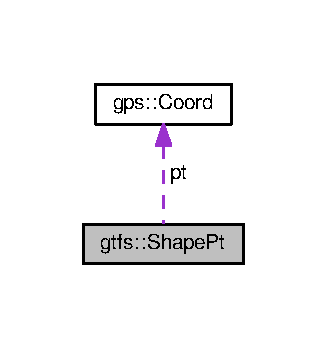
\includegraphics[width=157pt]{structgtfs_1_1ShapePt__coll__graph}
\end{center}
\end{figure}
\subsection*{Public Member Functions}
\begin{DoxyCompactItemize}
\item 
\hyperlink{structgtfs_1_1ShapePt_a34e7da183770e2ab8360e286596ff18a}{Shape\+Pt} (\hyperlink{classgps_1_1Coord}{gps\+::\+Coord} \hyperlink{structgtfs_1_1ShapePt_ab79eb8263213afd27be9b257fca8515a}{pt}, double distance)
\item 
\hyperlink{structgtfs_1_1ShapePt_a44b97d5fba5a7f1d0c7988dbe8748f85}{Shape\+Pt} (\hyperlink{classgps_1_1Coord}{gps\+::\+Coord} \hyperlink{structgtfs_1_1ShapePt_ab79eb8263213afd27be9b257fca8515a}{pt})
\end{DoxyCompactItemize}
\subsection*{Public Attributes}
\begin{DoxyCompactItemize}
\item 
\hyperlink{classgps_1_1Coord}{gps\+::\+Coord} \hyperlink{structgtfs_1_1ShapePt_ab79eb8263213afd27be9b257fca8515a}{pt}
\item 
double \hyperlink{structgtfs_1_1ShapePt_acb29ef40a33bee6b4000c31731e25073}{dist\+\_\+traveled}
\end{DoxyCompactItemize}


\subsection{Detailed Description}
A struct describing a single shape point. 

\subsection{Constructor \& Destructor Documentation}
\mbox{\Hypertarget{structgtfs_1_1ShapePt_a34e7da183770e2ab8360e286596ff18a}\label{structgtfs_1_1ShapePt_a34e7da183770e2ab8360e286596ff18a}} 
\index{gtfs\+::\+Shape\+Pt@{gtfs\+::\+Shape\+Pt}!Shape\+Pt@{Shape\+Pt}}
\index{Shape\+Pt@{Shape\+Pt}!gtfs\+::\+Shape\+Pt@{gtfs\+::\+Shape\+Pt}}
\subsubsection{\texorpdfstring{Shape\+Pt()}{ShapePt()}\hspace{0.1cm}{\footnotesize\ttfamily [1/2]}}
{\footnotesize\ttfamily gtfs\+::\+Shape\+Pt\+::\+Shape\+Pt (\begin{DoxyParamCaption}\item[{\hyperlink{classgps_1_1Coord}{gps\+::\+Coord}}]{pt,  }\item[{double}]{distance }\end{DoxyParamCaption})\hspace{0.3cm}{\ttfamily [inline]}}

Default constructor for a shape point, which defines a G\+PS location and how far into the shape that point is.


\begin{DoxyParams}{Parameters}
{\em pt} & G\+PS position of the point \\
\hline
{\em distance} & the point\textquotesingle{}s distance along the path \\
\hline
\end{DoxyParams}
\mbox{\Hypertarget{structgtfs_1_1ShapePt_a44b97d5fba5a7f1d0c7988dbe8748f85}\label{structgtfs_1_1ShapePt_a44b97d5fba5a7f1d0c7988dbe8748f85}} 
\index{gtfs\+::\+Shape\+Pt@{gtfs\+::\+Shape\+Pt}!Shape\+Pt@{Shape\+Pt}}
\index{Shape\+Pt@{Shape\+Pt}!gtfs\+::\+Shape\+Pt@{gtfs\+::\+Shape\+Pt}}
\subsubsection{\texorpdfstring{Shape\+Pt()}{ShapePt()}\hspace{0.1cm}{\footnotesize\ttfamily [2/2]}}
{\footnotesize\ttfamily gtfs\+::\+Shape\+Pt\+::\+Shape\+Pt (\begin{DoxyParamCaption}\item[{\hyperlink{classgps_1_1Coord}{gps\+::\+Coord}}]{pt }\end{DoxyParamCaption})\hspace{0.3cm}{\ttfamily [inline]}}

Constructor without distance. 
\begin{DoxyParams}{Parameters}
{\em pt} & G\+PS position of point. \\
\hline
\end{DoxyParams}


\subsection{Member Data Documentation}
\mbox{\Hypertarget{structgtfs_1_1ShapePt_acb29ef40a33bee6b4000c31731e25073}\label{structgtfs_1_1ShapePt_acb29ef40a33bee6b4000c31731e25073}} 
\index{gtfs\+::\+Shape\+Pt@{gtfs\+::\+Shape\+Pt}!dist\+\_\+traveled@{dist\+\_\+traveled}}
\index{dist\+\_\+traveled@{dist\+\_\+traveled}!gtfs\+::\+Shape\+Pt@{gtfs\+::\+Shape\+Pt}}
\subsubsection{\texorpdfstring{dist\+\_\+traveled}{dist\_traveled}}
{\footnotesize\ttfamily double gtfs\+::\+Shape\+Pt\+::dist\+\_\+traveled}

cumulative distance traveled along the shape \mbox{\Hypertarget{structgtfs_1_1ShapePt_ab79eb8263213afd27be9b257fca8515a}\label{structgtfs_1_1ShapePt_ab79eb8263213afd27be9b257fca8515a}} 
\index{gtfs\+::\+Shape\+Pt@{gtfs\+::\+Shape\+Pt}!pt@{pt}}
\index{pt@{pt}!gtfs\+::\+Shape\+Pt@{gtfs\+::\+Shape\+Pt}}
\subsubsection{\texorpdfstring{pt}{pt}}
{\footnotesize\ttfamily \hyperlink{classgps_1_1Coord}{gps\+::\+Coord} gtfs\+::\+Shape\+Pt\+::pt}

G\+PS coordinate of the point 

The documentation for this struct was generated from the following file\+:\begin{DoxyCompactItemize}
\item 
gtfs/gtfs.\+h\end{DoxyCompactItemize}

\hypertarget{structgtfs_1_1ShapeSegment}{}\section{gtfs\+:\+:Shape\+Segment Struct Reference}
\label{structgtfs_1_1ShapeSegment}\index{gtfs\+::\+Shape\+Segment@{gtfs\+::\+Shape\+Segment}}


{\ttfamily \#include $<$gtfs.\+h$>$}

\subsection*{Public Member Functions}
\begin{DoxyCompactItemize}
\item 
\hyperlink{structgtfs_1_1ShapeSegment_af1bdb1504d16a49ab6ac8ea34da59c5f}{Shape\+Segment} (std\+::shared\+\_\+ptr$<$ \hyperlink{classgtfs_1_1Segment}{Segment} $>$ \hyperlink{structgtfs_1_1ShapeSegment_a3253b76a15e2645f894a75be55006e09}{segment}, double distance)
\end{DoxyCompactItemize}
\subsection*{Public Attributes}
\begin{DoxyCompactItemize}
\item 
std\+::shared\+\_\+ptr$<$ \hyperlink{classgtfs_1_1Segment}{Segment} $>$ \hyperlink{structgtfs_1_1ShapeSegment_a3253b76a15e2645f894a75be55006e09}{segment}
\item 
double \hyperlink{structgtfs_1_1ShapeSegment_a64afdd03235b9bc256fc18652c6f9c47}{shape\+\_\+dist\+\_\+traveled}
\end{DoxyCompactItemize}


\subsection{Detailed Description}
A struct corresponding legs of a shape with segments.

The vector order == leg (0-\/based sequence). 

\subsection{Constructor \& Destructor Documentation}
\index{gtfs\+::\+Shape\+Segment@{gtfs\+::\+Shape\+Segment}!Shape\+Segment@{Shape\+Segment}}
\index{Shape\+Segment@{Shape\+Segment}!gtfs\+::\+Shape\+Segment@{gtfs\+::\+Shape\+Segment}}
\subsubsection[{\texorpdfstring{Shape\+Segment(std\+::shared\+\_\+ptr$<$ Segment $>$ segment, double distance)}{ShapeSegment(std::shared_ptr< Segment > segment, double distance)}}]{\setlength{\rightskip}{0pt plus 5cm}gtfs\+::\+Shape\+Segment\+::\+Shape\+Segment (
\begin{DoxyParamCaption}
\item[{std\+::shared\+\_\+ptr$<$ {\bf Segment} $>$}]{segment, }
\item[{double}]{distance}
\end{DoxyParamCaption}
)\hspace{0.3cm}{\ttfamily [inline]}}\hypertarget{structgtfs_1_1ShapeSegment_af1bdb1504d16a49ab6ac8ea34da59c5f}{}\label{structgtfs_1_1ShapeSegment_af1bdb1504d16a49ab6ac8ea34da59c5f}
Default constructor for a \hyperlink{classgtfs_1_1Shape}{Shape} \hyperlink{classgtfs_1_1Segment}{Segment}.

This is simply a relationship between a \hyperlink{classgtfs_1_1GTFS}{G\+T\+FS} S\+H\+A\+PE and it\textquotesingle{}s segment information. That is, it\textquotesingle{}s a \textquotesingle{}pivot table\textquotesingle{}.


\begin{DoxyParams}{Parameters}
{\em segment} & the segment ID \\
\hline
{\em distance} & how far into the overall shape this segment starts at \\
\hline
\end{DoxyParams}


\subsection{Member Data Documentation}
\index{gtfs\+::\+Shape\+Segment@{gtfs\+::\+Shape\+Segment}!segment@{segment}}
\index{segment@{segment}!gtfs\+::\+Shape\+Segment@{gtfs\+::\+Shape\+Segment}}
\subsubsection[{\texorpdfstring{segment}{segment}}]{\setlength{\rightskip}{0pt plus 5cm}std\+::shared\+\_\+ptr$<${\bf Segment}$>$ gtfs\+::\+Shape\+Segment\+::segment}\hypertarget{structgtfs_1_1ShapeSegment_a3253b76a15e2645f894a75be55006e09}{}\label{structgtfs_1_1ShapeSegment_a3253b76a15e2645f894a75be55006e09}
pointer to the segment \index{gtfs\+::\+Shape\+Segment@{gtfs\+::\+Shape\+Segment}!shape\+\_\+dist\+\_\+traveled@{shape\+\_\+dist\+\_\+traveled}}
\index{shape\+\_\+dist\+\_\+traveled@{shape\+\_\+dist\+\_\+traveled}!gtfs\+::\+Shape\+Segment@{gtfs\+::\+Shape\+Segment}}
\subsubsection[{\texorpdfstring{shape\+\_\+dist\+\_\+traveled}{shape_dist_traveled}}]{\setlength{\rightskip}{0pt plus 5cm}double gtfs\+::\+Shape\+Segment\+::shape\+\_\+dist\+\_\+traveled}\hypertarget{structgtfs_1_1ShapeSegment_a64afdd03235b9bc256fc18652c6f9c47}{}\label{structgtfs_1_1ShapeSegment_a64afdd03235b9bc256fc18652c6f9c47}
distance along route shape at beginning of this segment 

The documentation for this struct was generated from the following file\+:\begin{DoxyCompactItemize}
\item 
gtfs/gtfs.\+h\end{DoxyCompactItemize}

\hypertarget{classgtfs_1_1Stop}{}\section{gtfs\+:\+:Stop Class Reference}
\label{classgtfs_1_1Stop}\index{gtfs\+::\+Stop@{gtfs\+::\+Stop}}


{\ttfamily \#include $<$gtfs.\+h$>$}

\subsection*{Public Member Functions}
\begin{DoxyCompactItemize}
\item 
\hyperlink{classgtfs_1_1Stop_ac2654c54aaf615ad670c1f9c0c2fe729}{Stop} (std\+::string \&id, \hyperlink{classgps_1_1Coord}{gps\+::\+Coord} \&pos)
\item 
const std\+::string \& \hyperlink{classgtfs_1_1Stop_a95f4a615a6e06eed430a14d783557a29}{get\+\_\+id} (void) const
\item 
const \hyperlink{classgps_1_1Coord}{gps\+::\+Coord} \& \hyperlink{classgtfs_1_1Stop_acdd72b43e30c15819f16807b5c6a45d3}{get\+\_\+pos} (void) const
\end{DoxyCompactItemize}


\subsection{Detailed Description}
An object of this class represents a physical stop.

Stops have a position on a map, as well as dwell time parameters which can be implemented in the model at a later date to help differentiate busy and remote stops. 

\subsection{Constructor \& Destructor Documentation}
\mbox{\Hypertarget{classgtfs_1_1Stop_ac2654c54aaf615ad670c1f9c0c2fe729}\label{classgtfs_1_1Stop_ac2654c54aaf615ad670c1f9c0c2fe729}} 
\index{gtfs\+::\+Stop@{gtfs\+::\+Stop}!Stop@{Stop}}
\index{Stop@{Stop}!gtfs\+::\+Stop@{gtfs\+::\+Stop}}
\subsubsection{\texorpdfstring{Stop()}{Stop()}}
{\footnotesize\ttfamily gtfs\+::\+Stop\+::\+Stop (\begin{DoxyParamCaption}\item[{std\+::string \&}]{id,  }\item[{\hyperlink{classgps_1_1Coord}{gps\+::\+Coord} \&}]{pos }\end{DoxyParamCaption})}

Constructor for a stop object. 

\subsection{Member Function Documentation}
\mbox{\Hypertarget{classgtfs_1_1Stop_a95f4a615a6e06eed430a14d783557a29}\label{classgtfs_1_1Stop_a95f4a615a6e06eed430a14d783557a29}} 
\index{gtfs\+::\+Stop@{gtfs\+::\+Stop}!get\+\_\+id@{get\+\_\+id}}
\index{get\+\_\+id@{get\+\_\+id}!gtfs\+::\+Stop@{gtfs\+::\+Stop}}
\subsubsection{\texorpdfstring{get\+\_\+id()}{get\_id()}}
{\footnotesize\ttfamily const std\+::string\& gtfs\+::\+Stop\+::get\+\_\+id (\begin{DoxyParamCaption}\item[{void}]{ }\end{DoxyParamCaption}) const\hspace{0.3cm}{\ttfamily [inline]}}

\begin{DoxyReturn}{Returns}
the stop\textquotesingle{}s ID 
\end{DoxyReturn}
\mbox{\Hypertarget{classgtfs_1_1Stop_acdd72b43e30c15819f16807b5c6a45d3}\label{classgtfs_1_1Stop_acdd72b43e30c15819f16807b5c6a45d3}} 
\index{gtfs\+::\+Stop@{gtfs\+::\+Stop}!get\+\_\+pos@{get\+\_\+pos}}
\index{get\+\_\+pos@{get\+\_\+pos}!gtfs\+::\+Stop@{gtfs\+::\+Stop}}
\subsubsection{\texorpdfstring{get\+\_\+pos()}{get\_pos()}}
{\footnotesize\ttfamily const \hyperlink{classgps_1_1Coord}{gps\+::\+Coord}\& gtfs\+::\+Stop\+::get\+\_\+pos (\begin{DoxyParamCaption}\item[{void}]{ }\end{DoxyParamCaption}) const\hspace{0.3cm}{\ttfamily [inline]}}

\begin{DoxyReturn}{Returns}
the stop\textquotesingle{}s G\+PS position 
\end{DoxyReturn}


The documentation for this class was generated from the following files\+:\begin{DoxyCompactItemize}
\item 
gtfs/gtfs.\+h\item 
gtfs/Stop.\+cpp\end{DoxyCompactItemize}

\hypertarget{structgtfs_1_1StopTime}{}\section{gtfs\+:\+:Stop\+Time Struct Reference}
\label{structgtfs_1_1StopTime}\index{gtfs\+::\+Stop\+Time@{gtfs\+::\+Stop\+Time}}


{\ttfamily \#include $<$gtfs.\+h$>$}

\subsection*{Public Member Functions}
\begin{DoxyCompactItemize}
\item 
\hyperlink{structgtfs_1_1StopTime_adb27c1b3ad66cdc37e4a78338ad2b1a5}{Stop\+Time} (std\+::shared\+\_\+ptr$<$ \hyperlink{classgtfs_1_1Stop}{Stop} $>$ \hyperlink{structgtfs_1_1StopTime_a586702c54a1ad350d486c6639558b4ca}{stop}, std\+::string \&arrival, std\+::string \&departure)
\end{DoxyCompactItemize}
\subsection*{Public Attributes}
\begin{DoxyCompactItemize}
\item 
std\+::shared\+\_\+ptr$<$ \hyperlink{classgtfs_1_1Stop}{Stop} $>$ \hyperlink{structgtfs_1_1StopTime_a586702c54a1ad350d486c6639558b4ca}{stop}
\item 
boost\+::posix\+\_\+time\+::time\+\_\+duration \hyperlink{structgtfs_1_1StopTime_a994ec898edd96675200f759acd76a57c}{arrival\+\_\+time}
\item 
boost\+::posix\+\_\+time\+::time\+\_\+duration \hyperlink{structgtfs_1_1StopTime_ad11c398eca36ff99f0934883141de3c9}{departure\+\_\+time}
\item 
bool \hyperlink{structgtfs_1_1StopTime_af8cc780329a837a49a5d6af60b74b9bf}{layover}
\end{DoxyCompactItemize}


\subsection{Detailed Description}
A struct representing an instance of a trip arriving at a stop. 

\subsection{Constructor \& Destructor Documentation}
\index{gtfs\+::\+Stop\+Time@{gtfs\+::\+Stop\+Time}!Stop\+Time@{Stop\+Time}}
\index{Stop\+Time@{Stop\+Time}!gtfs\+::\+Stop\+Time@{gtfs\+::\+Stop\+Time}}
\subsubsection[{\texorpdfstring{Stop\+Time(std\+::shared\+\_\+ptr$<$ Stop $>$ stop, std\+::string \&arrival, std\+::string \&departure)}{StopTime(std::shared_ptr< Stop > stop, std::string &arrival, std::string &departure)}}]{\setlength{\rightskip}{0pt plus 5cm}gtfs\+::\+Stop\+Time\+::\+Stop\+Time (
\begin{DoxyParamCaption}
\item[{std\+::shared\+\_\+ptr$<$ {\bf Stop} $>$}]{stop, }
\item[{std\+::string \&}]{arrival, }
\item[{std\+::string \&}]{departure}
\end{DoxyParamCaption}
)\hspace{0.3cm}{\ttfamily [inline]}}\hypertarget{structgtfs_1_1StopTime_adb27c1b3ad66cdc37e4a78338ad2b1a5}{}\label{structgtfs_1_1StopTime_adb27c1b3ad66cdc37e4a78338ad2b1a5}
Constructor for a \hyperlink{structgtfs_1_1StopTime}{Stop\+Time} struct 

\subsection{Member Data Documentation}
\index{gtfs\+::\+Stop\+Time@{gtfs\+::\+Stop\+Time}!arrival\+\_\+time@{arrival\+\_\+time}}
\index{arrival\+\_\+time@{arrival\+\_\+time}!gtfs\+::\+Stop\+Time@{gtfs\+::\+Stop\+Time}}
\subsubsection[{\texorpdfstring{arrival\+\_\+time}{arrival_time}}]{\setlength{\rightskip}{0pt plus 5cm}boost\+::posix\+\_\+time\+::time\+\_\+duration gtfs\+::\+Stop\+Time\+::arrival\+\_\+time}\hypertarget{structgtfs_1_1StopTime_a994ec898edd96675200f759acd76a57c}{}\label{structgtfs_1_1StopTime_a994ec898edd96675200f759acd76a57c}
the scheduled arrival time \index{gtfs\+::\+Stop\+Time@{gtfs\+::\+Stop\+Time}!departure\+\_\+time@{departure\+\_\+time}}
\index{departure\+\_\+time@{departure\+\_\+time}!gtfs\+::\+Stop\+Time@{gtfs\+::\+Stop\+Time}}
\subsubsection[{\texorpdfstring{departure\+\_\+time}{departure_time}}]{\setlength{\rightskip}{0pt plus 5cm}boost\+::posix\+\_\+time\+::time\+\_\+duration gtfs\+::\+Stop\+Time\+::departure\+\_\+time}\hypertarget{structgtfs_1_1StopTime_ad11c398eca36ff99f0934883141de3c9}{}\label{structgtfs_1_1StopTime_ad11c398eca36ff99f0934883141de3c9}
the scheduled departure time \index{gtfs\+::\+Stop\+Time@{gtfs\+::\+Stop\+Time}!layover@{layover}}
\index{layover@{layover}!gtfs\+::\+Stop\+Time@{gtfs\+::\+Stop\+Time}}
\subsubsection[{\texorpdfstring{layover}{layover}}]{\setlength{\rightskip}{0pt plus 5cm}bool gtfs\+::\+Stop\+Time\+::layover}\hypertarget{structgtfs_1_1StopTime_af8cc780329a837a49a5d6af60b74b9bf}{}\label{structgtfs_1_1StopTime_af8cc780329a837a49a5d6af60b74b9bf}
if true, the stop is a layover and we assume the bus doesn\textquotesingle{}t leave until the scheduled departure time \index{gtfs\+::\+Stop\+Time@{gtfs\+::\+Stop\+Time}!stop@{stop}}
\index{stop@{stop}!gtfs\+::\+Stop\+Time@{gtfs\+::\+Stop\+Time}}
\subsubsection[{\texorpdfstring{stop}{stop}}]{\setlength{\rightskip}{0pt plus 5cm}std\+::shared\+\_\+ptr$<${\bf Stop}$>$ gtfs\+::\+Stop\+Time\+::stop}\hypertarget{structgtfs_1_1StopTime_a586702c54a1ad350d486c6639558b4ca}{}\label{structgtfs_1_1StopTime_a586702c54a1ad350d486c6639558b4ca}
pointer to the stop 

The documentation for this struct was generated from the following file\+:\begin{DoxyCompactItemize}
\item 
gtfs/gtfs.\+h\end{DoxyCompactItemize}

\hypertarget{classgtfs_1_1Trip}{}\section{gtfs\+:\+:Trip Class Reference}
\label{classgtfs_1_1Trip}\index{gtfs\+::\+Trip@{gtfs\+::\+Trip}}


{\ttfamily \#include $<$gtfs.\+h$>$}



Inheritance diagram for gtfs\+:\+:Trip\+:\nopagebreak
\begin{figure}[H]
\begin{center}
\leavevmode
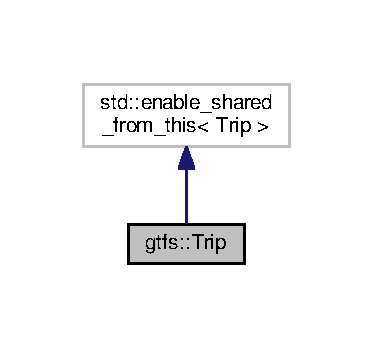
\includegraphics[width=179pt]{classgtfs_1_1Trip__inherit__graph}
\end{center}
\end{figure}


Collaboration diagram for gtfs\+:\+:Trip\+:\nopagebreak
\begin{figure}[H]
\begin{center}
\leavevmode
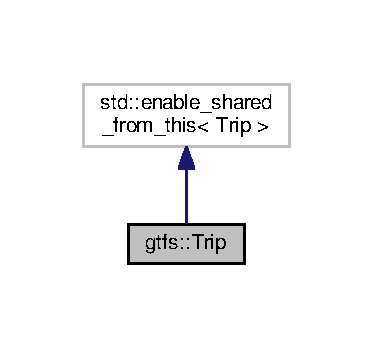
\includegraphics[width=179pt]{classgtfs_1_1Trip__coll__graph}
\end{center}
\end{figure}
\subsection*{Public Member Functions}
\begin{DoxyCompactItemize}
\item 
\hyperlink{classgtfs_1_1Trip_a3014ee32fdb5abd550ad20088c91aae6}{Trip} (std\+::string \&id, std\+::shared\+\_\+ptr$<$ \hyperlink{classgtfs_1_1Route}{Route} $>$ route)
\item 
std\+::string \hyperlink{classgtfs_1_1Trip_ac4c80cbf34f7c715104cc1c33b082f58}{get\+\_\+id} (void) const
\item 
std\+::shared\+\_\+ptr$<$ \hyperlink{classgtfs_1_1Route}{Route} $>$ \hyperlink{classgtfs_1_1Trip_a2b6cc135946d7e7db7bb35951987e35c}{get\+\_\+route} (void)
\end{DoxyCompactItemize}


\subsection{Detailed Description}
An object of this class represents a unique T\+R\+IP in the \hyperlink{classgtfs_1_1GTFS}{G\+T\+FS} schedule.

A trip is an instance of a route that occurs at a specific time of day. It has a sequence of stop times. 

\subsection{Constructor \& Destructor Documentation}
\mbox{\Hypertarget{classgtfs_1_1Trip_a3014ee32fdb5abd550ad20088c91aae6}\label{classgtfs_1_1Trip_a3014ee32fdb5abd550ad20088c91aae6}} 
\index{gtfs\+::\+Trip@{gtfs\+::\+Trip}!Trip@{Trip}}
\index{Trip@{Trip}!gtfs\+::\+Trip@{gtfs\+::\+Trip}}
\subsubsection{\texorpdfstring{Trip()}{Trip()}}
{\footnotesize\ttfamily gtfs\+::\+Trip\+::\+Trip (\begin{DoxyParamCaption}\item[{std\+::string \&}]{id,  }\item[{std\+::shared\+\_\+ptr$<$ \hyperlink{classgtfs_1_1Route}{Route} $>$}]{route }\end{DoxyParamCaption})}

Constructor for a trip object, taking an ID and a route pointer. \begin{DoxyReturn}{Returns}
\mbox{[}description\mbox{]} 
\end{DoxyReturn}


\subsection{Member Function Documentation}
\mbox{\Hypertarget{classgtfs_1_1Trip_ac4c80cbf34f7c715104cc1c33b082f58}\label{classgtfs_1_1Trip_ac4c80cbf34f7c715104cc1c33b082f58}} 
\index{gtfs\+::\+Trip@{gtfs\+::\+Trip}!get\+\_\+id@{get\+\_\+id}}
\index{get\+\_\+id@{get\+\_\+id}!gtfs\+::\+Trip@{gtfs\+::\+Trip}}
\subsubsection{\texorpdfstring{get\+\_\+id()}{get\_id()}}
{\footnotesize\ttfamily std\+::string gtfs\+::\+Trip\+::get\+\_\+id (\begin{DoxyParamCaption}\item[{void}]{ }\end{DoxyParamCaption}) const\hspace{0.3cm}{\ttfamily [inline]}}

\begin{DoxyReturn}{Returns}
the trip\textquotesingle{}s ID 
\end{DoxyReturn}
\mbox{\Hypertarget{classgtfs_1_1Trip_a2b6cc135946d7e7db7bb35951987e35c}\label{classgtfs_1_1Trip_a2b6cc135946d7e7db7bb35951987e35c}} 
\index{gtfs\+::\+Trip@{gtfs\+::\+Trip}!get\+\_\+route@{get\+\_\+route}}
\index{get\+\_\+route@{get\+\_\+route}!gtfs\+::\+Trip@{gtfs\+::\+Trip}}
\subsubsection{\texorpdfstring{get\+\_\+route()}{get\_route()}}
{\footnotesize\ttfamily std\+::shared\+\_\+ptr$<$\hyperlink{classgtfs_1_1Route}{Route}$>$ gtfs\+::\+Trip\+::get\+\_\+route (\begin{DoxyParamCaption}\item[{void}]{ }\end{DoxyParamCaption})\hspace{0.3cm}{\ttfamily [inline]}}

\begin{DoxyReturn}{Returns}
a pointer to the trip\textquotesingle{}s route 
\end{DoxyReturn}


The documentation for this class was generated from the following files\+:\begin{DoxyCompactItemize}
\item 
gtfs/gtfs.\+h\item 
gtfs/Trip.\+cpp\end{DoxyCompactItemize}

\hypertarget{classsampling_1_1uniform}{}\section{sampling\+:\+:uniform Class Reference}
\label{classsampling_1_1uniform}\index{sampling\+::uniform@{sampling\+::uniform}}


{\ttfamily \#include $<$sampling.\+h$>$}

\subsection*{Public Member Functions}
\begin{DoxyCompactItemize}
\item 
\hyperlink{classsampling_1_1uniform_a414a98d445c6a07bbe78ea677db19f69}{uniform} ()
\item 
\hyperlink{classsampling_1_1uniform_a67fa371e5e843209c83d584c33dd8957}{uniform} (double a, double b)
\item 
double \hyperlink{classsampling_1_1uniform_a9fcb1597ca643fb1c2184f6febc69b0d}{pdf} (double x)
\item 
double \hyperlink{classsampling_1_1uniform_a30fa2f2be90f2f9f2d46069540019fb4}{pdf\+\_\+log} (double x)
\item 
double \hyperlink{classsampling_1_1uniform_aee0b21aec2c50cdb6d926d5c3890d695}{rand} (\hyperlink{classsampling_1_1RNG}{sampling\+::\+R\+NG} \&rng)
\end{DoxyCompactItemize}


\subsection{Detailed Description}
Class used for Uniform distributions.

(Log) P\+DF and random variables 

\subsection{Constructor \& Destructor Documentation}
\mbox{\Hypertarget{classsampling_1_1uniform_a414a98d445c6a07bbe78ea677db19f69}\label{classsampling_1_1uniform_a414a98d445c6a07bbe78ea677db19f69}} 
\index{sampling\+::uniform@{sampling\+::uniform}!uniform@{uniform}}
\index{uniform@{uniform}!sampling\+::uniform@{sampling\+::uniform}}
\subsubsection{\texorpdfstring{uniform()}{uniform()}\hspace{0.1cm}{\footnotesize\ttfamily [1/2]}}
{\footnotesize\ttfamily sampling\+::uniform\+::uniform (\begin{DoxyParamCaption}{ }\end{DoxyParamCaption})}

Default constructor for a standard uniform, U(0,1) \mbox{\Hypertarget{classsampling_1_1uniform_a67fa371e5e843209c83d584c33dd8957}\label{classsampling_1_1uniform_a67fa371e5e843209c83d584c33dd8957}} 
\index{sampling\+::uniform@{sampling\+::uniform}!uniform@{uniform}}
\index{uniform@{uniform}!sampling\+::uniform@{sampling\+::uniform}}
\subsubsection{\texorpdfstring{uniform()}{uniform()}\hspace{0.1cm}{\footnotesize\ttfamily [2/2]}}
{\footnotesize\ttfamily sampling\+::uniform\+::uniform (\begin{DoxyParamCaption}\item[{double}]{a,  }\item[{double}]{b }\end{DoxyParamCaption})}

General constructor for a uniform U(a,b) 

\subsection{Member Function Documentation}
\mbox{\Hypertarget{classsampling_1_1uniform_a9fcb1597ca643fb1c2184f6febc69b0d}\label{classsampling_1_1uniform_a9fcb1597ca643fb1c2184f6febc69b0d}} 
\index{sampling\+::uniform@{sampling\+::uniform}!pdf@{pdf}}
\index{pdf@{pdf}!sampling\+::uniform@{sampling\+::uniform}}
\subsubsection{\texorpdfstring{pdf()}{pdf()}}
{\footnotesize\ttfamily double sampling\+::uniform\+::pdf (\begin{DoxyParamCaption}\item[{double}]{x }\end{DoxyParamCaption})}

Computes the P\+DF for a given value of x 
\begin{DoxyParams}{Parameters}
{\em x} & the x value to evaluate \\
\hline
\end{DoxyParams}
\begin{DoxyReturn}{Returns}
the probability density function at x 
\end{DoxyReturn}
\mbox{\Hypertarget{classsampling_1_1uniform_a30fa2f2be90f2f9f2d46069540019fb4}\label{classsampling_1_1uniform_a30fa2f2be90f2f9f2d46069540019fb4}} 
\index{sampling\+::uniform@{sampling\+::uniform}!pdf\+\_\+log@{pdf\+\_\+log}}
\index{pdf\+\_\+log@{pdf\+\_\+log}!sampling\+::uniform@{sampling\+::uniform}}
\subsubsection{\texorpdfstring{pdf\+\_\+log()}{pdf\_log()}}
{\footnotesize\ttfamily double sampling\+::uniform\+::pdf\+\_\+log (\begin{DoxyParamCaption}\item[{double}]{x }\end{DoxyParamCaption})}

Returns the log P\+DF for a given x 
\begin{DoxyParams}{Parameters}
{\em x} & x value to evaluate \\
\hline
\end{DoxyParams}
\begin{DoxyReturn}{Returns}
log probability density at x 
\end{DoxyReturn}
\mbox{\Hypertarget{classsampling_1_1uniform_aee0b21aec2c50cdb6d926d5c3890d695}\label{classsampling_1_1uniform_aee0b21aec2c50cdb6d926d5c3890d695}} 
\index{sampling\+::uniform@{sampling\+::uniform}!rand@{rand}}
\index{rand@{rand}!sampling\+::uniform@{sampling\+::uniform}}
\subsubsection{\texorpdfstring{rand()}{rand()}}
{\footnotesize\ttfamily double sampling\+::uniform\+::rand (\begin{DoxyParamCaption}\item[{\hyperlink{classsampling_1_1RNG}{sampling\+::\+R\+NG} \&}]{rng }\end{DoxyParamCaption})}

Sample a random observation from the given uniform distribution 
\begin{DoxyParams}{Parameters}
{\em rng} & reference to a \hyperlink{classsampling_1_1RNG}{R\+NG} \\
\hline
\end{DoxyParams}
\begin{DoxyReturn}{Returns}
a random value 
\end{DoxyReturn}


The documentation for this class was generated from the following files\+:\begin{DoxyCompactItemize}
\item 
sampling/sampling.\+h\item 
sampling/uniform.\+cpp\end{DoxyCompactItemize}

\hypertarget{classgtfs_1_1Vehicle}{}\section{gtfs\+:\+:Vehicle Class Reference}
\label{classgtfs_1_1Vehicle}\index{gtfs\+::\+Vehicle@{gtfs\+::\+Vehicle}}


{\ttfamily \#include $<$gtfs.\+h$>$}

\subsection*{Public Member Functions}
\begin{DoxyCompactItemize}
\item 
\hyperlink{classgtfs_1_1Vehicle_a8838934149e47eeb7160f1755012dcd4}{Vehicle} (std\+::string id, \hyperlink{classsampling_1_1RNG}{sampling\+::\+R\+NG} \&rng)
\item 
\hyperlink{classgtfs_1_1Vehicle_a12765a61077b4be7e65ab67b63eb9fcc}{Vehicle} (std\+::string id, unsigned int n, \hyperlink{classsampling_1_1RNG}{sampling\+::\+R\+NG} \&rng)
\item 
\hyperlink{classgtfs_1_1Vehicle_a08c7450dd0df9406f78b30be044d27d8}{$\sim$\+Vehicle} ()
\item 
std\+::string \hyperlink{classgtfs_1_1Vehicle_a6b388986c9ed4af1eb86f13a3d2de8e0}{get\+\_\+id} () const
\item 
std\+::vector$<$ \hyperlink{classgtfs_1_1Particle}{Particle} $>$ \& \hyperlink{classgtfs_1_1Vehicle_a7b12b079c68880f00f532ca25858c368}{get\+\_\+particles} ()
\item 
int \hyperlink{classgtfs_1_1Vehicle_a23c0a191559e4066423d5f3cbfb70b46}{get\+\_\+delta} () const
\item 
\mbox{\Hypertarget{classgtfs_1_1Vehicle_aab490aeda8084cfcb8de29f0aedaa416}\label{classgtfs_1_1Vehicle_aab490aeda8084cfcb8de29f0aedaa416}} 
void {\bfseries update} (void)
\item 
void \hyperlink{classgtfs_1_1Vehicle_a50ae70c92d958437a2196b0ce81acff0}{update} (const transit\+\_\+realtime\+::\+Vehicle\+Position \&vp)
\item 
void \hyperlink{classgtfs_1_1Vehicle_a4cc25a17473bf7bccc39b37ef5d7c956}{update} (const transit\+\_\+realtime\+::\+Trip\+Update \&tu)
\item 
unsigned long \hyperlink{classgtfs_1_1Vehicle_aa9087e973a9821f384ec47f51bdcedc7}{allocate\+\_\+id} ()
\item 
void \hyperlink{classgtfs_1_1Vehicle_a8367fc70a64b7e596422f880dbff1193}{resample} (\hyperlink{classsampling_1_1RNG}{sampling\+::\+R\+NG} \&rng)
\end{DoxyCompactItemize}
\subsection*{Public Attributes}
\begin{DoxyCompactItemize}
\item 
unsigned int \hyperlink{classgtfs_1_1Vehicle_aa21babc8423abf92bbdf5e0748444f44}{n\+\_\+particles}
\item 
unsigned long \hyperlink{classgtfs_1_1Vehicle_aab535dd9953f9650e2adc351965779b1}{next\+\_\+id}
\end{DoxyCompactItemize}


\subsection{Detailed Description}
Transit vehicle class

A representation of a physical transit vehicle (i.\+e., a bus), including the most recent data associated with that vehicle (G\+PS location, arrival/departure time, etc).

Vehicles are initialized with an ID, so it is not editable. 

\subsection{Constructor \& Destructor Documentation}
\mbox{\Hypertarget{classgtfs_1_1Vehicle_a8838934149e47eeb7160f1755012dcd4}\label{classgtfs_1_1Vehicle_a8838934149e47eeb7160f1755012dcd4}} 
\index{gtfs\+::\+Vehicle@{gtfs\+::\+Vehicle}!Vehicle@{Vehicle}}
\index{Vehicle@{Vehicle}!gtfs\+::\+Vehicle@{gtfs\+::\+Vehicle}}
\subsubsection{\texorpdfstring{Vehicle()}{Vehicle()}\hspace{0.1cm}{\footnotesize\ttfamily [1/2]}}
{\footnotesize\ttfamily gtfs\+::\+Vehicle\+::\+Vehicle (\begin{DoxyParamCaption}\item[{std\+::string}]{id,  }\item[{\hyperlink{classsampling_1_1RNG}{sampling\+::\+R\+NG} \&}]{rng }\end{DoxyParamCaption})}

Create a \hyperlink{classgtfs_1_1Vehicle}{Vehicle} object with given ID.

Vehicles are created with a default number of particles.


\begin{DoxyParams}{Parameters}
{\em vehicle\+\_\+id} & the ID of the vehicle as given in the G\+T\+FS feed \\
\hline
\end{DoxyParams}
\mbox{\Hypertarget{classgtfs_1_1Vehicle_a12765a61077b4be7e65ab67b63eb9fcc}\label{classgtfs_1_1Vehicle_a12765a61077b4be7e65ab67b63eb9fcc}} 
\index{gtfs\+::\+Vehicle@{gtfs\+::\+Vehicle}!Vehicle@{Vehicle}}
\index{Vehicle@{Vehicle}!gtfs\+::\+Vehicle@{gtfs\+::\+Vehicle}}
\subsubsection{\texorpdfstring{Vehicle()}{Vehicle()}\hspace{0.1cm}{\footnotesize\ttfamily [2/2]}}
{\footnotesize\ttfamily gtfs\+::\+Vehicle\+::\+Vehicle (\begin{DoxyParamCaption}\item[{std\+::string}]{id,  }\item[{unsigned int}]{n,  }\item[{\hyperlink{classsampling_1_1RNG}{sampling\+::\+R\+NG} \&}]{rng }\end{DoxyParamCaption})}

Create a vehicle with specified number of particles, and ID.


\begin{DoxyParams}{Parameters}
{\em id} & the ID of the vehicle as given in the G\+T\+FS feed \\
\hline
{\em n} & integer specifying the number of particles to initialize the vehicle with \\
\hline
\end{DoxyParams}
\mbox{\Hypertarget{classgtfs_1_1Vehicle_a08c7450dd0df9406f78b30be044d27d8}\label{classgtfs_1_1Vehicle_a08c7450dd0df9406f78b30be044d27d8}} 
\index{gtfs\+::\+Vehicle@{gtfs\+::\+Vehicle}!````~Vehicle@{$\sim$\+Vehicle}}
\index{````~Vehicle@{$\sim$\+Vehicle}!gtfs\+::\+Vehicle@{gtfs\+::\+Vehicle}}
\subsubsection{\texorpdfstring{$\sim$\+Vehicle()}{~Vehicle()}}
{\footnotesize\ttfamily gtfs\+::\+Vehicle\+::$\sim$\+Vehicle (\begin{DoxyParamCaption}{ }\end{DoxyParamCaption})}

Desctructor for a vehicle object, ensuring all particles are deleted too. 

\subsection{Member Function Documentation}
\mbox{\Hypertarget{classgtfs_1_1Vehicle_aa9087e973a9821f384ec47f51bdcedc7}\label{classgtfs_1_1Vehicle_aa9087e973a9821f384ec47f51bdcedc7}} 
\index{gtfs\+::\+Vehicle@{gtfs\+::\+Vehicle}!allocate\+\_\+id@{allocate\+\_\+id}}
\index{allocate\+\_\+id@{allocate\+\_\+id}!gtfs\+::\+Vehicle@{gtfs\+::\+Vehicle}}
\subsubsection{\texorpdfstring{allocate\+\_\+id()}{allocate\_id()}}
{\footnotesize\ttfamily unsigned long gtfs\+::\+Vehicle\+::allocate\+\_\+id (\begin{DoxyParamCaption}{ }\end{DoxyParamCaption})}

To ensure particles have unique ID\textquotesingle{}s (within a vehicle), the next ID is incremended when requested by a new particle.

\begin{DoxyReturn}{Returns}
the ID for the next particle. 
\end{DoxyReturn}
\mbox{\Hypertarget{classgtfs_1_1Vehicle_a23c0a191559e4066423d5f3cbfb70b46}\label{classgtfs_1_1Vehicle_a23c0a191559e4066423d5f3cbfb70b46}} 
\index{gtfs\+::\+Vehicle@{gtfs\+::\+Vehicle}!get\+\_\+delta@{get\+\_\+delta}}
\index{get\+\_\+delta@{get\+\_\+delta}!gtfs\+::\+Vehicle@{gtfs\+::\+Vehicle}}
\subsubsection{\texorpdfstring{get\+\_\+delta()}{get\_delta()}}
{\footnotesize\ttfamily int gtfs\+::\+Vehicle\+::get\+\_\+delta (\begin{DoxyParamCaption}{ }\end{DoxyParamCaption}) const}

\begin{DoxyReturn}{Returns}
time in seconds since the previous observation 
\end{DoxyReturn}
\mbox{\Hypertarget{classgtfs_1_1Vehicle_a6b388986c9ed4af1eb86f13a3d2de8e0}\label{classgtfs_1_1Vehicle_a6b388986c9ed4af1eb86f13a3d2de8e0}} 
\index{gtfs\+::\+Vehicle@{gtfs\+::\+Vehicle}!get\+\_\+id@{get\+\_\+id}}
\index{get\+\_\+id@{get\+\_\+id}!gtfs\+::\+Vehicle@{gtfs\+::\+Vehicle}}
\subsubsection{\texorpdfstring{get\+\_\+id()}{get\_id()}}
{\footnotesize\ttfamily std\+::string gtfs\+::\+Vehicle\+::get\+\_\+id (\begin{DoxyParamCaption}{ }\end{DoxyParamCaption}) const}

\begin{DoxyReturn}{Returns}
ID of vehicle 
\end{DoxyReturn}
\mbox{\Hypertarget{classgtfs_1_1Vehicle_a7b12b079c68880f00f532ca25858c368}\label{classgtfs_1_1Vehicle_a7b12b079c68880f00f532ca25858c368}} 
\index{gtfs\+::\+Vehicle@{gtfs\+::\+Vehicle}!get\+\_\+particles@{get\+\_\+particles}}
\index{get\+\_\+particles@{get\+\_\+particles}!gtfs\+::\+Vehicle@{gtfs\+::\+Vehicle}}
\subsubsection{\texorpdfstring{get\+\_\+particles()}{get\_particles()}}
{\footnotesize\ttfamily std\+::vector$<$ \hyperlink{classgtfs_1_1Particle}{gtfs\+::\+Particle} $>$ \& gtfs\+::\+Vehicle\+::get\+\_\+particles (\begin{DoxyParamCaption}{ }\end{DoxyParamCaption})}

\begin{DoxyReturn}{Returns}
vector of particle references (so they can be mofidied ...) 
\end{DoxyReturn}
\mbox{\Hypertarget{classgtfs_1_1Vehicle_a8367fc70a64b7e596422f880dbff1193}\label{classgtfs_1_1Vehicle_a8367fc70a64b7e596422f880dbff1193}} 
\index{gtfs\+::\+Vehicle@{gtfs\+::\+Vehicle}!resample@{resample}}
\index{resample@{resample}!gtfs\+::\+Vehicle@{gtfs\+::\+Vehicle}}
\subsubsection{\texorpdfstring{resample()}{resample()}}
{\footnotesize\ttfamily void gtfs\+::\+Vehicle\+::resample (\begin{DoxyParamCaption}\item[{\hyperlink{classsampling_1_1RNG}{sampling\+::\+R\+NG} \&}]{rng }\end{DoxyParamCaption})}

Perform weighted resampling with replacement.

Use the computed particle weights to resample, with replacement, the particles associated with the vehicle. \mbox{\Hypertarget{classgtfs_1_1Vehicle_a50ae70c92d958437a2196b0ce81acff0}\label{classgtfs_1_1Vehicle_a50ae70c92d958437a2196b0ce81acff0}} 
\index{gtfs\+::\+Vehicle@{gtfs\+::\+Vehicle}!update@{update}}
\index{update@{update}!gtfs\+::\+Vehicle@{gtfs\+::\+Vehicle}}
\subsubsection{\texorpdfstring{update()}{update()}\hspace{0.1cm}{\footnotesize\ttfamily [1/2]}}
{\footnotesize\ttfamily void gtfs\+::\+Vehicle\+::update (\begin{DoxyParamCaption}\item[{const transit\+\_\+realtime\+::\+Vehicle\+Position \&}]{vp }\end{DoxyParamCaption})}

Update the location of the vehicle object.

This does N\+OT trigger a particle update, as we may need to also insert Trip\+Updates later. Check that the trip\+\_\+id is the same, otherwise set {\ttfamily newtrip = false}


\begin{DoxyParams}{Parameters}
{\em vp} & a vehicle position from the realtime feed \\
\hline
\end{DoxyParams}
\mbox{\Hypertarget{classgtfs_1_1Vehicle_a4cc25a17473bf7bccc39b37ef5d7c956}\label{classgtfs_1_1Vehicle_a4cc25a17473bf7bccc39b37ef5d7c956}} 
\index{gtfs\+::\+Vehicle@{gtfs\+::\+Vehicle}!update@{update}}
\index{update@{update}!gtfs\+::\+Vehicle@{gtfs\+::\+Vehicle}}
\subsubsection{\texorpdfstring{update()}{update()}\hspace{0.1cm}{\footnotesize\ttfamily [2/2]}}
{\footnotesize\ttfamily void gtfs\+::\+Vehicle\+::update (\begin{DoxyParamCaption}\item[{const transit\+\_\+realtime\+::\+Trip\+Update \&}]{vp }\end{DoxyParamCaption})}

Add \hyperlink{classgtfs_1_1Stop}{Stop} Time Updates to the vehicle object.

This does N\+OT trigger a particle update, as we may need to also insert Vehicle\+Positions later.


\begin{DoxyParams}{Parameters}
{\em vp} & a vehicle position from the realtime feed \\
\hline
\end{DoxyParams}


\subsection{Member Data Documentation}
\mbox{\Hypertarget{classgtfs_1_1Vehicle_aa21babc8423abf92bbdf5e0748444f44}\label{classgtfs_1_1Vehicle_aa21babc8423abf92bbdf5e0748444f44}} 
\index{gtfs\+::\+Vehicle@{gtfs\+::\+Vehicle}!n\+\_\+particles@{n\+\_\+particles}}
\index{n\+\_\+particles@{n\+\_\+particles}!gtfs\+::\+Vehicle@{gtfs\+::\+Vehicle}}
\subsubsection{\texorpdfstring{n\+\_\+particles}{n\_particles}}
{\footnotesize\ttfamily unsigned int gtfs\+::\+Vehicle\+::n\+\_\+particles}

the number of particles that will be created in the next sample \mbox{\Hypertarget{classgtfs_1_1Vehicle_aab535dd9953f9650e2adc351965779b1}\label{classgtfs_1_1Vehicle_aab535dd9953f9650e2adc351965779b1}} 
\index{gtfs\+::\+Vehicle@{gtfs\+::\+Vehicle}!next\+\_\+id@{next\+\_\+id}}
\index{next\+\_\+id@{next\+\_\+id}!gtfs\+::\+Vehicle@{gtfs\+::\+Vehicle}}
\subsubsection{\texorpdfstring{next\+\_\+id}{next\_id}}
{\footnotesize\ttfamily unsigned long gtfs\+::\+Vehicle\+::next\+\_\+id}

the ID of the next particle to be created 

The documentation for this class was generated from the following files\+:\begin{DoxyCompactItemize}
\item 
gtfs/gtfs.\+h\item 
gtfs/Vehicle.\+cpp\end{DoxyCompactItemize}

\chapter{File Documentation}
\hypertarget{load__gtfs_8cpp}{}\section{src/load\+\_\+gtfs.cpp File Reference}
\label{load__gtfs_8cpp}\index{src/load\+\_\+gtfs.\+cpp@{src/load\+\_\+gtfs.\+cpp}}
{\ttfamily \#include $<$iostream$>$}\\*
{\ttfamily \#include $<$vector$>$}\\*
{\ttfamily \#include $<$stdlib.\+h$>$}\\*
{\ttfamily \#include $<$fstream$>$}\\*
{\ttfamily \#include $<$algorithm$>$}\\*
{\ttfamily \#include $<$boost/program\+\_\+options.\+hpp$>$}\\*
{\ttfamily \#include $<$sqlite3.\+h$>$}\\*
{\ttfamily \#include \char`\"{}gps.\+h\char`\"{}}\\*
{\ttfamily \#include \char`\"{}gtfs.\+h\char`\"{}}\\*
{\ttfamily \#include \char`\"{}json.\+hpp\char`\"{}}\\*
Include dependency graph for load\+\_\+gtfs.\+cpp\+:
\nopagebreak
\begin{figure}[H]
\begin{center}
\leavevmode
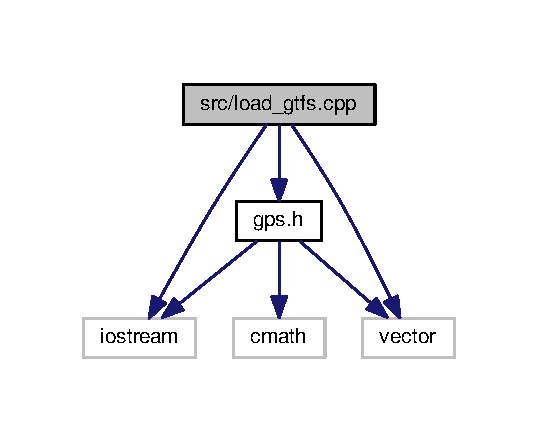
\includegraphics[width=350pt]{load__gtfs_8cpp__incl}
\end{center}
\end{figure}
\subsection*{Classes}
\begin{DoxyCompactItemize}
\item 
struct \hyperlink{structSplit}{Split}
\end{DoxyCompactItemize}
\subsection*{Functions}
\begin{DoxyCompactItemize}
\item 
int \hyperlink{load__gtfs_8cpp_acc289d9bfee4c154322662aef55c5438}{system} (std\+::string const \&s)
\item 
void \hyperlink{load__gtfs_8cpp_a54ef9ab4a1985152c9cf7ec290fbea2d}{import\+\_\+intersections} (sqlite3 $\ast$db, std\+::vector$<$ std\+::string $>$ files)
\item 
void \hyperlink{load__gtfs_8cpp_a2f86801b49d8f0b1649a9edc0e197172}{set\+\_\+distances} (sqlite3 $\ast$db)
\item 
std\+::vector$<$ \hyperlink{structSplit}{Split} $>$ \hyperlink{load__gtfs_8cpp_af82110f83438bd672ded68a2451e69f7}{find\+\_\+intersections} (std\+::shared\+\_\+ptr$<$ \hyperlink{classgtfs_1_1Shape}{gtfs\+::\+Shape} $>$ shape, std\+::vector$<$ \hyperlink{classgtfs_1_1Intersection}{gtfs\+::\+Intersection} $>$ \&intersections)
\item 
void {\bfseries segment\+\_\+shapes} (sqlite3 $\ast$db)\hypertarget{load__gtfs_8cpp_a4c73441dc3489abcadf91f57dd472673}{}\label{load__gtfs_8cpp_a4c73441dc3489abcadf91f57dd472673}

\item 
void {\bfseries calculate\+\_\+stop\+\_\+distances} (std\+::string \&dbname)\hypertarget{load__gtfs_8cpp_afc0ec9cd72ffe92b7aacb7c58aeea6b3}{}\label{load__gtfs_8cpp_afc0ec9cd72ffe92b7aacb7c58aeea6b3}

\item 
int \hyperlink{load__gtfs_8cpp_a0ddf1224851353fc92bfbff6f499fa97}{main} (int argc, char $\ast$argv\mbox{[}$\,$\mbox{]})
\end{DoxyCompactItemize}


\subsection{Detailed Description}
Load the most recent G\+T\+FS static data from Auckland Transport.

This program will populate the supplied database with the most recent version of the G\+T\+FS static feed from Auckland Transport.

Segmentation will take place, in which shapes are split at intersections. Routes will be compared to existing routes, and if there are no changes the segments will simply be duplicated; otherwise new segments will be created.

\begin{DoxyAuthor}{Author}
Tom Elliott \href{mailto:tom.elliott@auckland.ac.nz}{\tt tom.\+elliott@auckland.\+ac.\+nz} 
\end{DoxyAuthor}
\begin{DoxyVersion}{Version}
0.\+0.\+1 
\end{DoxyVersion}


\subsection{Function Documentation}
\index{load\+\_\+gtfs.\+cpp@{load\+\_\+gtfs.\+cpp}!find\+\_\+intersections@{find\+\_\+intersections}}
\index{find\+\_\+intersections@{find\+\_\+intersections}!load\+\_\+gtfs.\+cpp@{load\+\_\+gtfs.\+cpp}}
\subsubsection[{\texorpdfstring{find\+\_\+intersections(std\+::shared\+\_\+ptr$<$ gtfs\+::\+Shape $>$ shape, std\+::vector$<$ gtfs\+::\+Intersection $>$ \&intersections)}{find_intersections(std::shared_ptr< gtfs::Shape > shape, std::vector< gtfs::Intersection > &intersections)}}]{\setlength{\rightskip}{0pt plus 5cm}std\+::vector$<$ {\bf Split} $>$ find\+\_\+intersections (
\begin{DoxyParamCaption}
\item[{std\+::shared\+\_\+ptr$<$ {\bf gtfs\+::\+Shape} $>$}]{shape, }
\item[{std\+::vector$<$ {\bf gtfs\+::\+Intersection} $>$ \&}]{intersections}
\end{DoxyParamCaption}
)}\hypertarget{load__gtfs_8cpp_af82110f83438bd672ded68a2451e69f7}{}\label{load__gtfs_8cpp_af82110f83438bd672ded68a2451e69f7}
Find intersections along a path (multiple if it loops etc). 
\begin{DoxyParams}{Parameters}
{\em path} & path to look through \\
\hline
{\em intersections} & possible intersections \\
\hline
\end{DoxyParams}
\begin{DoxyReturn}{Returns}
vector of split points 
\end{DoxyReturn}
\index{load\+\_\+gtfs.\+cpp@{load\+\_\+gtfs.\+cpp}!import\+\_\+intersections@{import\+\_\+intersections}}
\index{import\+\_\+intersections@{import\+\_\+intersections}!load\+\_\+gtfs.\+cpp@{load\+\_\+gtfs.\+cpp}}
\subsubsection[{\texorpdfstring{import\+\_\+intersections(sqlite3 $\ast$db, std\+::vector$<$ std\+::string $>$ files)}{import_intersections(sqlite3 *db, std::vector< std::string > files)}}]{\setlength{\rightskip}{0pt plus 5cm}void import\+\_\+intersections (
\begin{DoxyParamCaption}
\item[{sqlite3 $\ast$}]{db, }
\item[{std\+::vector$<$ std\+::string $>$}]{files}
\end{DoxyParamCaption}
)}\hypertarget{load__gtfs_8cpp_a54ef9ab4a1985152c9cf7ec290fbea2d}{}\label{load__gtfs_8cpp_a54ef9ab4a1985152c9cf7ec290fbea2d}
Import insersections from a J\+S\+ON file into the database.

Additionally, clusters of \char`\"{}points\char`\"{} belonging to the same intersection are combined into a single object.


\begin{DoxyParams}{Parameters}
{\em db} & the database to use \\
\hline
{\em files} & the files to load intersections from \\
\hline
\end{DoxyParams}
\index{load\+\_\+gtfs.\+cpp@{load\+\_\+gtfs.\+cpp}!main@{main}}
\index{main@{main}!load\+\_\+gtfs.\+cpp@{load\+\_\+gtfs.\+cpp}}
\subsubsection[{\texorpdfstring{main(int argc, char $\ast$argv[])}{main(int argc, char *argv[])}}]{\setlength{\rightskip}{0pt plus 5cm}int main (
\begin{DoxyParamCaption}
\item[{int}]{argc, }
\item[{char $\ast$}]{argv\mbox{[}$\,$\mbox{]}}
\end{DoxyParamCaption}
)}\hypertarget{load__gtfs_8cpp_a0ddf1224851353fc92bfbff6f499fa97}{}\label{load__gtfs_8cpp_a0ddf1224851353fc92bfbff6f499fa97}
Loads G\+T\+FS file into database and segments as necessary.


\begin{DoxyParams}{Parameters}
{\em argc} & number of command line arguments \\
\hline
{\em argv} & arguments \\
\hline
\end{DoxyParams}
\begin{DoxyReturn}{Returns}
0 if everything went OK; 1 if it didn\textquotesingle{}t 
\end{DoxyReturn}
database connection to use \index{load\+\_\+gtfs.\+cpp@{load\+\_\+gtfs.\+cpp}!set\+\_\+distances@{set\+\_\+distances}}
\index{set\+\_\+distances@{set\+\_\+distances}!load\+\_\+gtfs.\+cpp@{load\+\_\+gtfs.\+cpp}}
\subsubsection[{\texorpdfstring{set\+\_\+distances(sqlite3 $\ast$db)}{set_distances(sqlite3 *db)}}]{\setlength{\rightskip}{0pt plus 5cm}void set\+\_\+distances (
\begin{DoxyParamCaption}
\item[{sqlite3 $\ast$}]{db}
\end{DoxyParamCaption}
)}\hypertarget{load__gtfs_8cpp_a2f86801b49d8f0b1649a9edc0e197172}{}\label{load__gtfs_8cpp_a2f86801b49d8f0b1649a9edc0e197172}
Set distance in database for segments and stops

To reduce reads, perform all at once, route by route. For each route
\begin{DoxyItemize}
\item load associated shape data into a Shape object
\item find intersections (in path order)
\begin{DoxyItemize}
\item (use code from segment\+\_\+shape fn)
\end{DoxyItemize}
\item load stops
\item travel along path computing distance traveled for each stop and intersection along the way
\end{DoxyItemize}


\begin{DoxyParams}{Parameters}
{\em db} & the database to use \\
\hline
\end{DoxyParams}
\index{load\+\_\+gtfs.\+cpp@{load\+\_\+gtfs.\+cpp}!system@{system}}
\index{system@{system}!load\+\_\+gtfs.\+cpp@{load\+\_\+gtfs.\+cpp}}
\subsubsection[{\texorpdfstring{system(std\+::string const \&s)}{system(std::string const &s)}}]{\setlength{\rightskip}{0pt plus 5cm}int system (
\begin{DoxyParamCaption}
\item[{std\+::string const \&}]{s}
\end{DoxyParamCaption}
)}\hypertarget{load__gtfs_8cpp_acc289d9bfee4c154322662aef55c5438}{}\label{load__gtfs_8cpp_acc289d9bfee4c154322662aef55c5438}
A \hyperlink{load__gtfs_8cpp_acc289d9bfee4c154322662aef55c5438}{system()} command that takes a std\+::string instead of a char. 
\begin{DoxyParams}{Parameters}
{\em s} & The command to run. \\
\hline
\end{DoxyParams}
\begin{DoxyReturn}{Returns}
The return value from the system command. 
\end{DoxyReturn}

\hypertarget{transit__network__model_8cpp}{}\section{src/transit\+\_\+network\+\_\+model.cpp File Reference}
\label{transit__network__model_8cpp}\index{src/transit\+\_\+network\+\_\+model.\+cpp@{src/transit\+\_\+network\+\_\+model.\+cpp}}
{\ttfamily \#include $<$iostream$>$}\\*
{\ttfamily \#include $<$memory$>$}\\*
{\ttfamily \#include $<$vector$>$}\\*
{\ttfamily \#include $<$gtfs.\+h$>$}\\*
Include dependency graph for transit\+\_\+network\+\_\+model.\+cpp\+:
\nopagebreak
\begin{figure}[H]
\begin{center}
\leavevmode
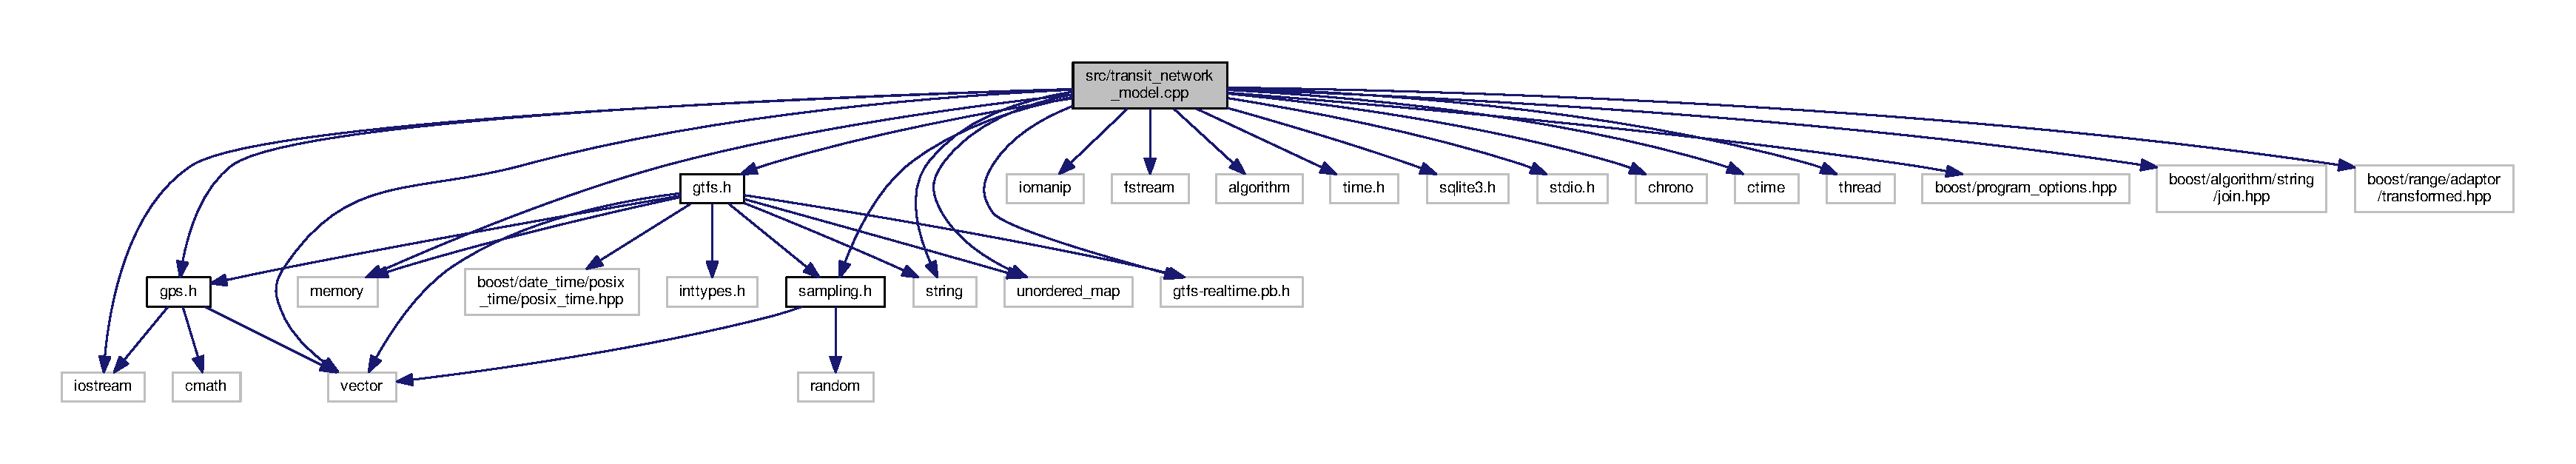
\includegraphics[width=350pt]{transit__network__model_8cpp__incl}
\end{center}
\end{figure}
\subsection*{Functions}
\begin{DoxyCompactItemize}
\item 
int \hyperlink{transit__network__model_8cpp_a0ddf1224851353fc92bfbff6f499fa97}{main} (int argc, char $\ast$argv\mbox{[}$\,$\mbox{]})
\end{DoxyCompactItemize}


\subsection{Detailed Description}
\begin{DoxyAuthor}{Author}
Tom Elliott \href{mailto:tom.elliott@auckland.ac.nz}{\tt tom.\+elliott@auckland.\+ac.\+nz} 
\end{DoxyAuthor}
\begin{DoxyVersion}{Version}
0.\+0.\+1 
\end{DoxyVersion}


\subsection{Function Documentation}
\index{transit\+\_\+network\+\_\+model.\+cpp@{transit\+\_\+network\+\_\+model.\+cpp}!main@{main}}
\index{main@{main}!transit\+\_\+network\+\_\+model.\+cpp@{transit\+\_\+network\+\_\+model.\+cpp}}
\subsubsection[{\texorpdfstring{main(int argc, char $\ast$argv[])}{main(int argc, char *argv[])}}]{\setlength{\rightskip}{0pt plus 5cm}int main (
\begin{DoxyParamCaption}
\item[{int}]{argc, }
\item[{char $\ast$}]{argv\mbox{[}$\,$\mbox{]}}
\end{DoxyParamCaption}
)}\hypertarget{transit__network__model_8cpp_a0ddf1224851353fc92bfbff6f499fa97}{}\label{transit__network__model_8cpp_a0ddf1224851353fc92bfbff6f499fa97}
Transit Network Model\+: a realtime model running indefinitely (while (true) \{ ... \})

Cycles through latest vehicles in the Realtime Feed, and updates/creates accordingly.


\begin{DoxyParams}{Parameters}
{\em argc} & number of command line arguments \\
\hline
{\em argv} & argument vector \\
\hline
\end{DoxyParams}
\begin{DoxyReturn}{Returns}
int 0 (although this will never happen because of the while forever loop) 
\end{DoxyReturn}

%--- End generated contents ---

% Index
\backmatter
\newpage
\phantomsection
\clearemptydoublepage
\addcontentsline{toc}{chapter}{Index}
\printindex

\end{document}
